\chapter{Architectural design}

\section{Overview}

In the S\&C application, five high-level components can be distinguished: the web server, the application server, the DBMS, the email service, and the browser interface.

The web server main objective is to deliver web pages upon user requests.
The application server is the main component of the system, as it contains every piece of business logic required to satisfy the goals specified in the RASD document.
The role of the DBMS is the usual, which is providing interaction with a database by executing command operations.
The email service is used to validate the user account at sign up time, since the verification link is sent via email.
Lastly, the browser interface is the application, in the form of web pages, that is reachable by the user from a browser.

\section{Components view}

\begin{enumerate}[label=\textbf{C\arabic* -}]

\item \htitle{Browser interface}
This is the the web application used by the client, which is reachable by any browser.
The full range of operations that it provides can only be used after the authentication process, performed by the authentication service, results successful.
It allows both students and companies to perform a certain set of actions based on the type of user.

\item \htitle{Web server}
This is the intermediary between the frontend and the backend.
Its purpose is to manage the browser UI pages independently and transparently from the point of view of the other servers components.
The web server main tasks are the static resources delivery and the web pages content retrieval and forwarding.
After receiving an HTTP request, the web server retrieves from the application server the data needed to fill the corresponding HTML template, which are then both returned to the user, along with the static style assets.

\item \htitle{DMBS}
The DBMS, which manages the DB containing all the data that the platform utilizes, stays on a separate machine.
It is then the query service component that, by providing the necessary SQL queries to other components, allows the application server to reach for the stored data.

\item \htitle{Email server}
The email server represents the external machines that the email service reaches in order to send messages.
Those machines are property of the actual email providers, but they show how the application server email service component can utilize them via their APIs.

\item \htitle{Request dispatcher}
The web server processes incoming HTTP requests by calling the appropriate application server component.
The components are responsible for retrieving the necessary data that the web server uses to populate the HTML template, which is then returned to the user.
Since different web pages may require data from different components, the request dispatcher ensures that each request is routed to the correct application server component.

\item \htitle{Authentication service}
This component provides the set of procedures required to handle the authentication of a user into the system.
It manages the log in and sign up phases.

\item \htitle{Email service}
The main goal of this component is to implement all the procedures that the server requires in order to send email messages to the user.
Mainly, this component allows the authentication service to send a verification email when handling the sign up of a user.

\item \htitle{Notification service}
The purpose of this component is to collect and manage all the notifications that a user receives.
It defines the notification types and allows other components to easily send them.

\item \htitle{Query service}
This service acts as a mediator between the server components and the DBMS.
It uses the DBMS APIs to implement a set of functions which have the sole purpose of manipulating the database or retrieving information from it.

\item \htitle{Recommendation service}
This service provides the algorithms necessary for finding suitable advertisements and candidates.
These are called when the user opens the feed in the home page, or when looking for strong matches that are to be notified.

\item \htitle{Suggestion service}
This service provides the algorithms necessary for evaluating the user profiles, in order to propose enhancements.
These are called by the profile manager component when the user provides new profile information.

\item \htitle{Profile manager}
Users must be able to insert and edit their profile information.
Validity checks and DB updates are performed by this component.
The query service and the suggestion service APIs are used when data is to be updated.

\item \htitle{Enrollment manager}
This component manages all the selection process phases, from the student application request to the start of the internship.
It also handles the questionnaires that companies send to students to fill in.

\item \htitle{Internship manager}
This component handles the operations that the internship may allow or require when it is in the ongoing status.
Along initializing and interrupting the internship, it permits users to visualize its annex information.

\item \htitle{Complaint manager}
This component allows students and companies to send complaints regarding an ongoing internship, hence allowing the university to visualize and handle them.
Since complaints must have a valid reference to an ongoing internship, the internship manager component APIs are here used.

\item \htitle{Feedback manager}
When an internship ends, both parties are requested to fill in a feedback form.
This component handles this operation, by sending, receiving and acting accordingly to the feedback forms content.
Since feedback forms must have a valid reference to an internship that has concluded, the internship manager component APIs are here used.

\end{enumerate}

\begin{figure}[H]
    \centering
    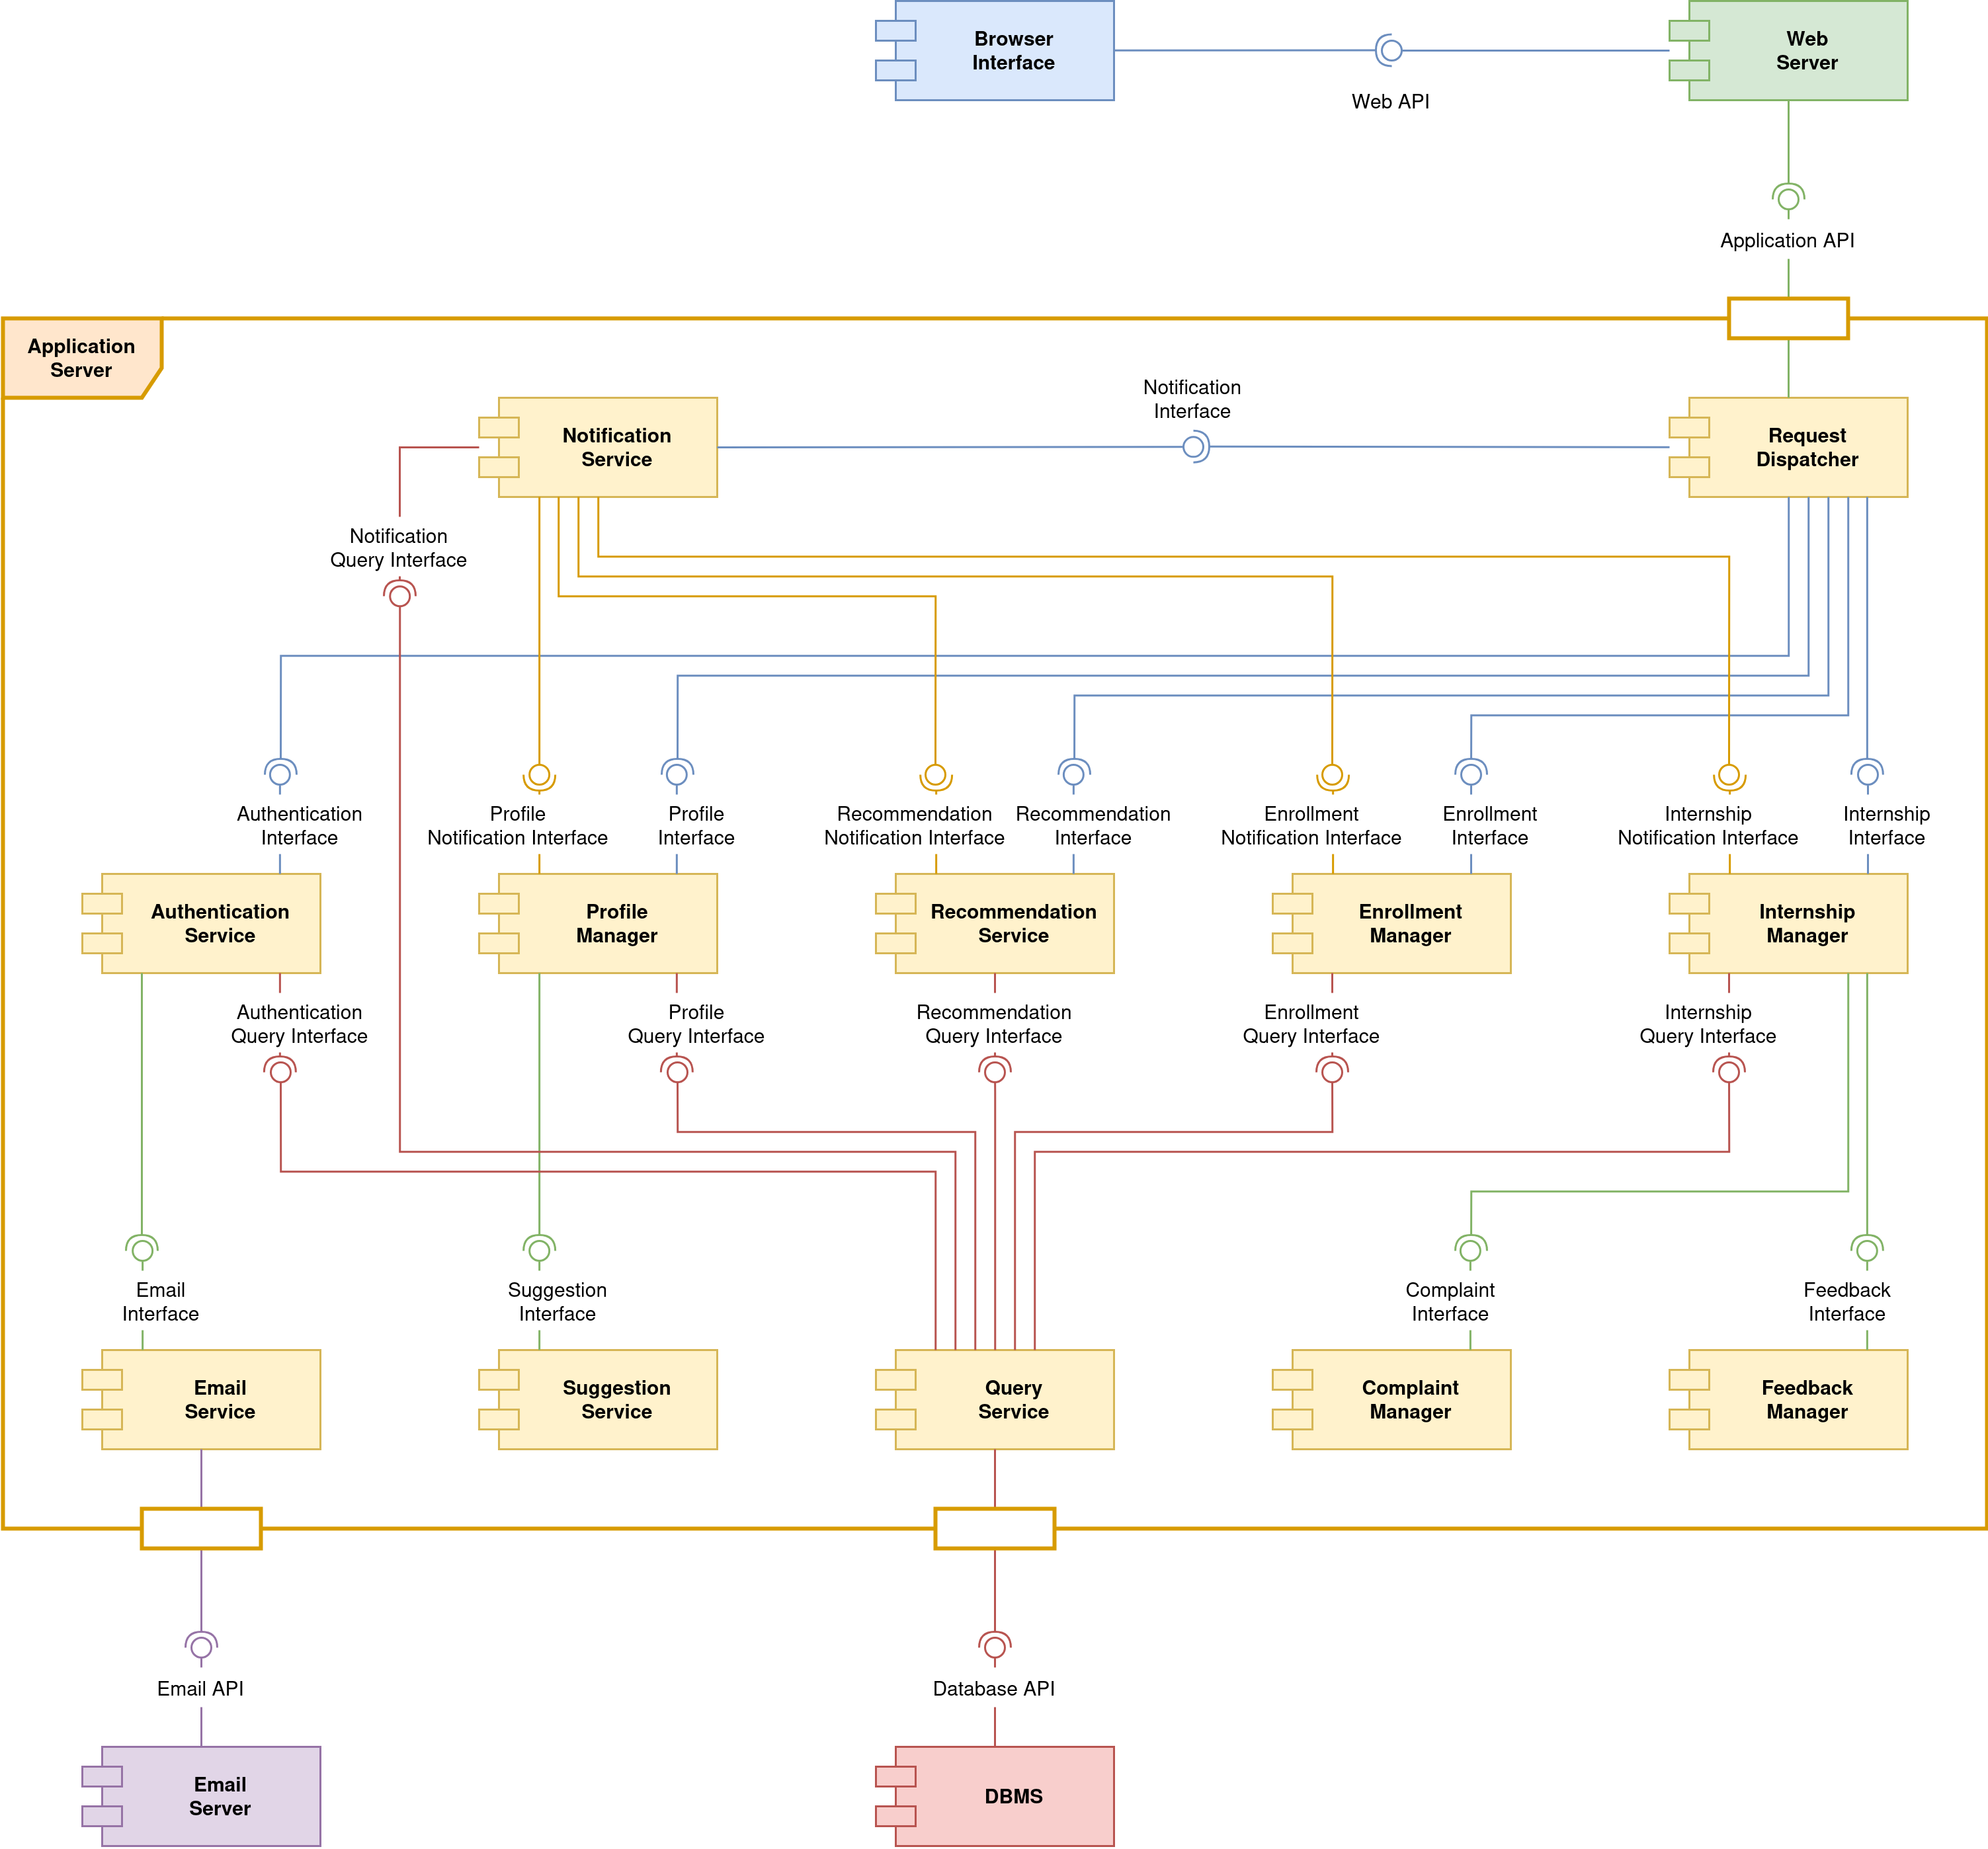
\includegraphics[width=0.8\linewidth]{../assets/components-diagrams/components-diagram.png}
\end{figure}

\subsection{Logical description of data}

The following diagram presents the logical design of the database, illustrated through an entity-relationship (ER) model.
The diagram defines the entities, their attributes, and the relationships between them, providing a structured and coherent representation of the system data organization.

The design ensures clarity in how information is managed, emphasizing integrity, consistency, and minimal redundancy.
It serves as a comprehensive framework for understanding the logical structure of the data and its interactions within the system.

\begin{figure}[H]
    \centering
    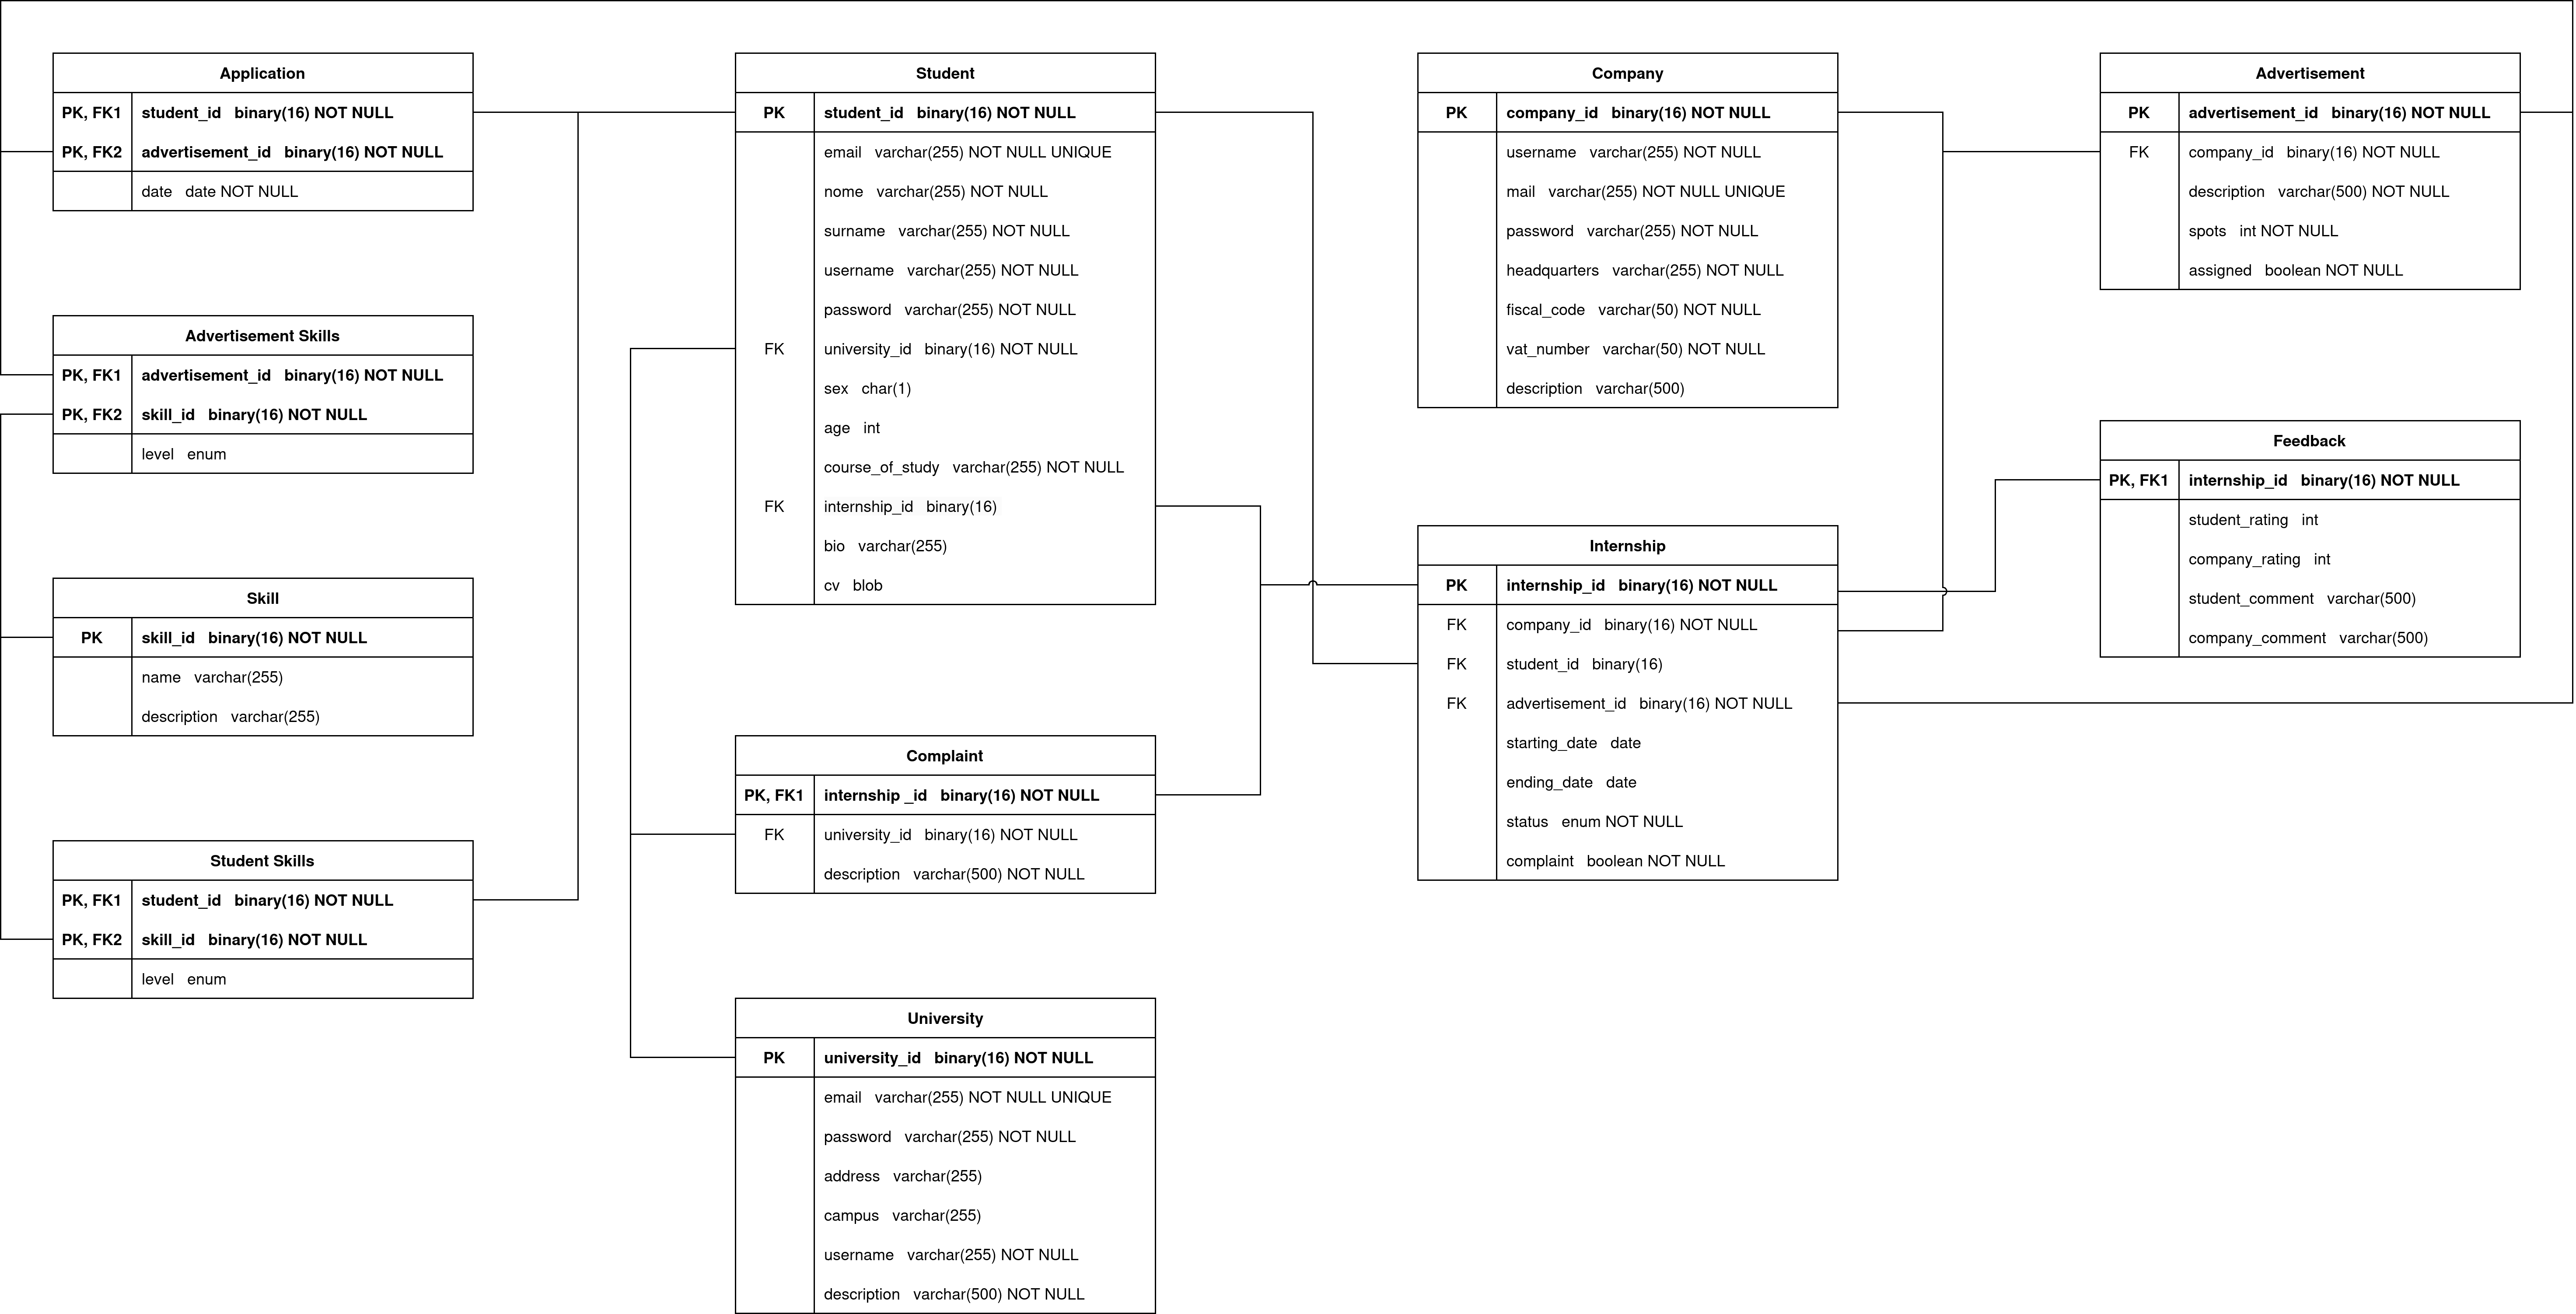
\includegraphics[width=0.8\linewidth]{../assets/er-diagrams/er-diagram.png}
\end{figure}

\section{Deployment view}

The following diagram shows the deployment view of the system.
It illustrates the distribution of the components on the different nodes, and how they communicate between each others.

The system is composed of four tiers, one for the client frontend and three for the server fullstack processes: the client tier, the web tier, the application tier and the data tier.
The client tier corresponds to the web browser, which is required by the user to access the application.
The web tier represents the web server, which is used to handle incoming user requests and to return web pages and their content.
The application tier corresponds to the application server, that is used to execute the business logic and to communicate with the database.
The data tier is composed of the database, which is used to store all the data that the application server may require.

The email service is a set of external APIs used by the application to send emails to the users.

Moreover, since the platform will potentially need to manage a lot of concurrent users, the implementation of load balancers can help distribute the load among multiple servers.
This allows the application to be more scalable, since it eases the addition of other servers to handle an increasing load.
Those are placed between the client and the web server, and between the web server and the application server.

Lastly, to protect the application from external attacks, multiple firewalls are in use to filter the traffic.
In particular, those are placed between the client and the web server, between the web servers and the application server, before the database, and between the application server and the provider's email server.
This allows the application to execute in a more secure environment, since the firewalls will filter the traffic before it reaches the designated component.

\begin{figure}[H]
    \centering
    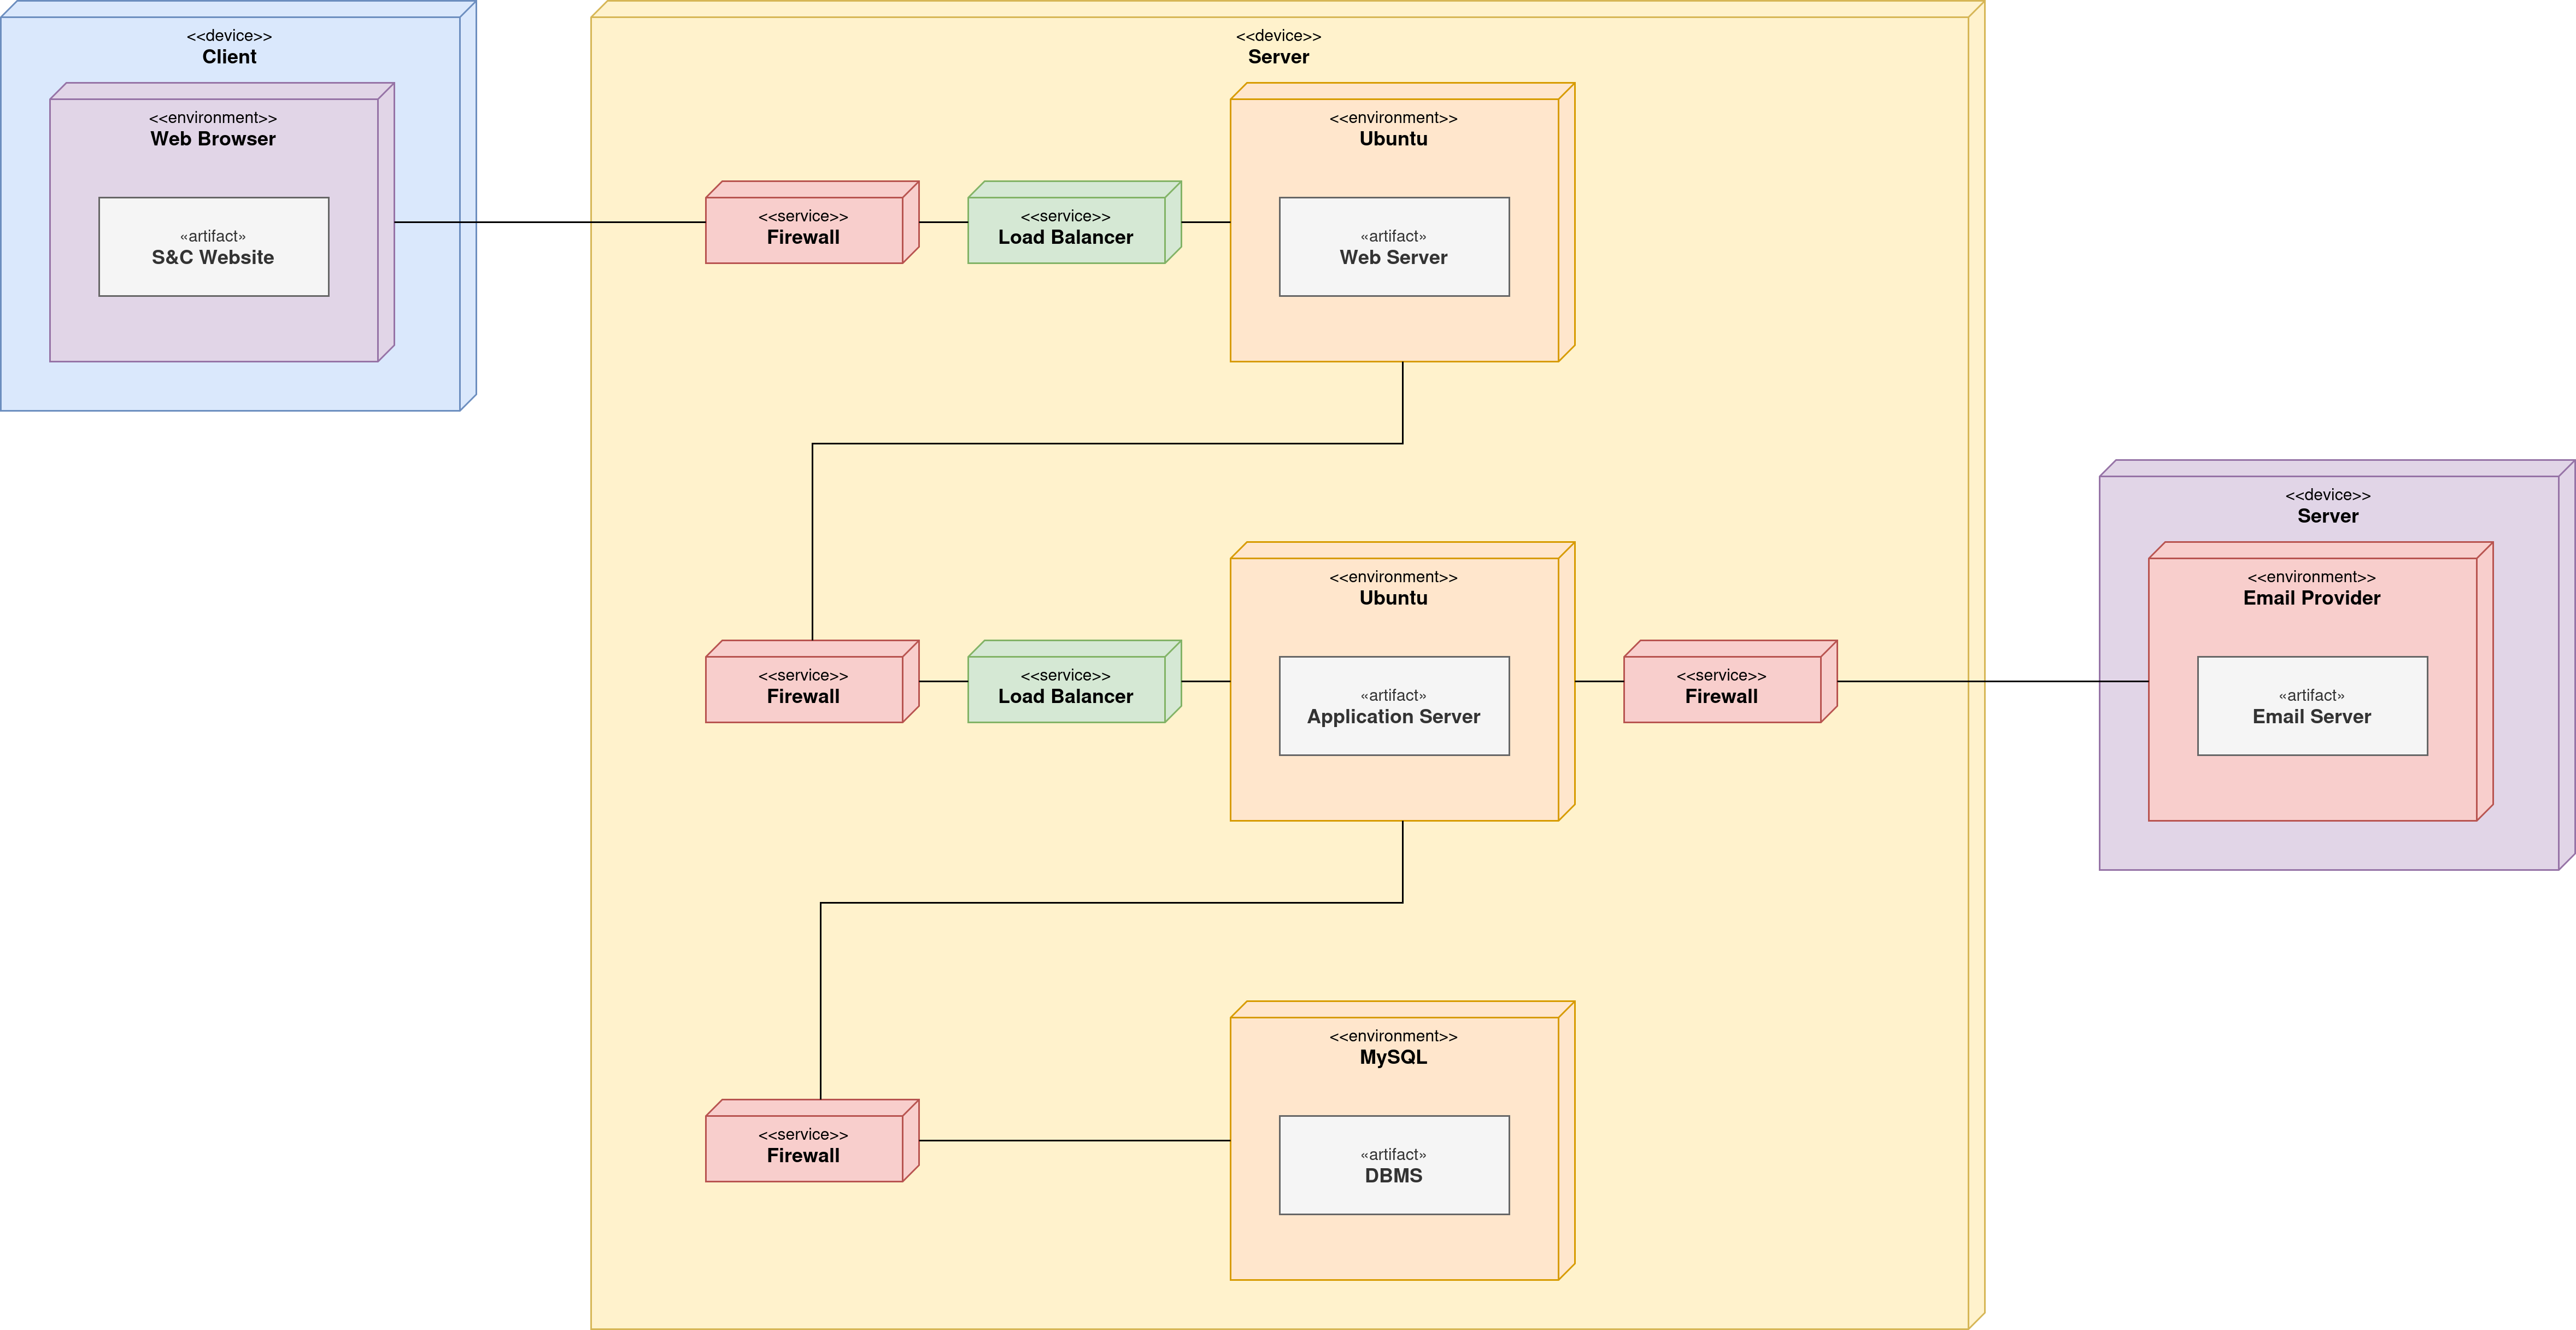
\includegraphics[width=0.8\linewidth]{../assets/deployment-diagrams/deployment-diagram.png}
\end{figure}

\section{Runtime view}

This section contains the sequence diagrams of the most important operations of the system.
The diagrams include the component described in the previous sections, and the external components that are involved in the operations.

\begin{enumerate}[label=\textbf{RV\arabic* -}]

\item \subsubsection{StudentSignsUp}

To register into the system, the user fills in the registration form and submits it.
The registration form fields vary based on whether signing up it is a student or a company.
The whole process is mainly handled by the authentication service component, that interacts with the query service to validate the information and to insert the new user into the DB.
The application server checks that information is valid, and that the user is not already registered.
Then, the system will insert the user into the DB and send an email to the user.
The email contains a link with the verification code.
The user, by clicking on the link, confirms the registration.

\begin{figure}[H]
    \centering
    \fcolorbox{black}{white}{
        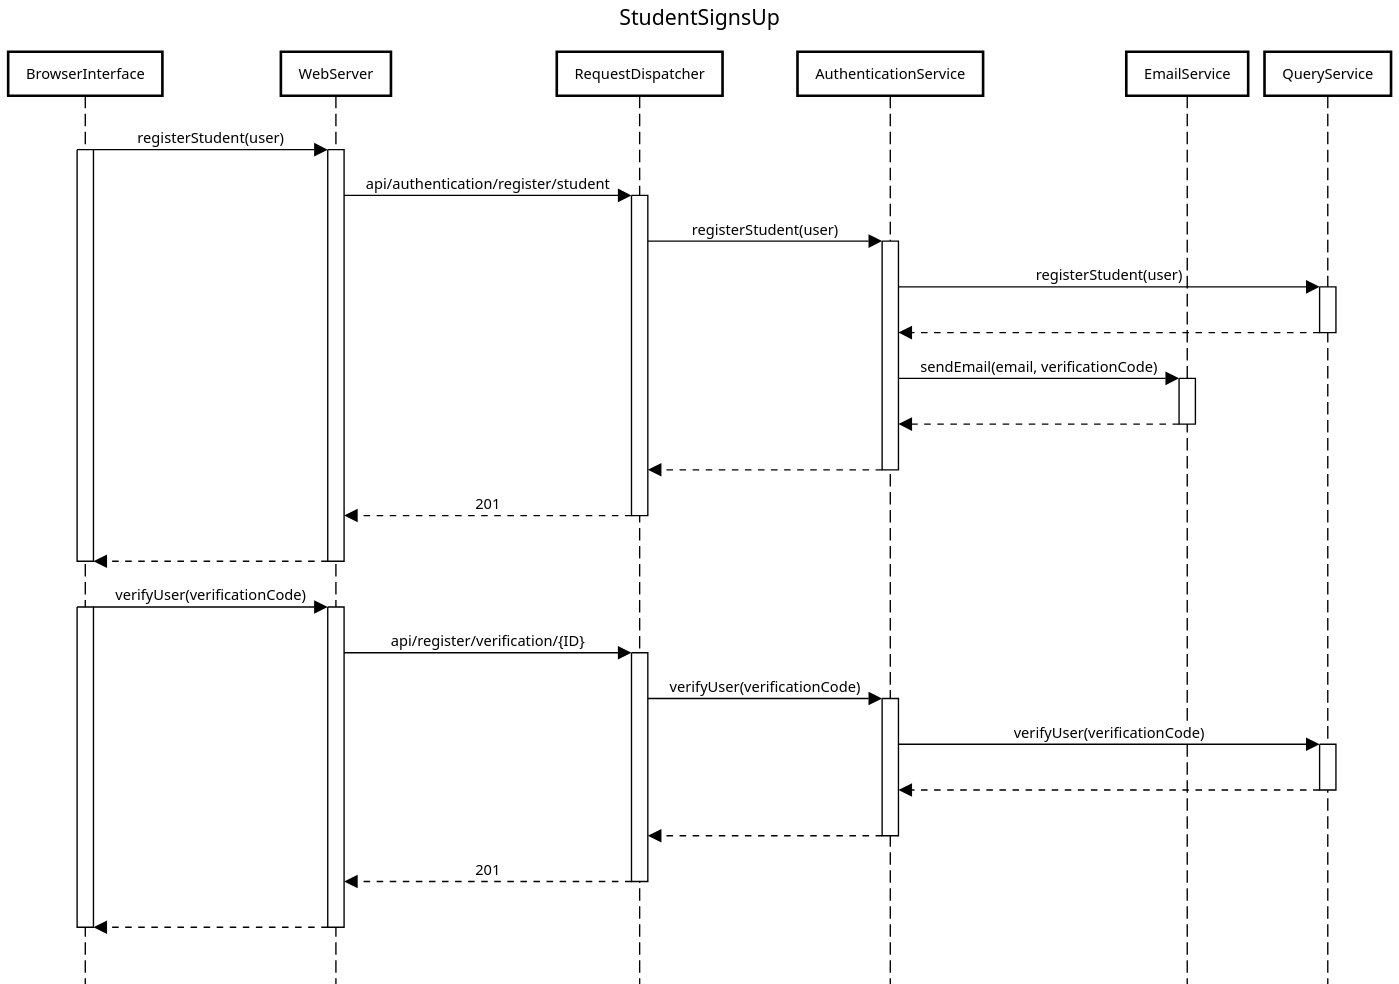
\includegraphics[width=0.8\linewidth]{../assets/runtime-views/StudentSignsUp.png}
    }
\end{figure}

\item \subsubsection{CompanySignsUp}

To register into the system, the user fills in the registration form and submits it.
The registration form fields vary based on whether signing up it is a student or a company.
The whole process is mainly handled by the authentication service component, that interacts with the query service to validate the information and to insert the new user into the DB.
The application server checks that information is valid, and that the user is not already registered.
Then, the system will insert the user into the DB and send an email to the user.
The email contains a link with the verification code.
The user, by clicking on the link, confirms the registration.

\begin{figure}[H]
    \centering
    \fcolorbox{black}{white}{
        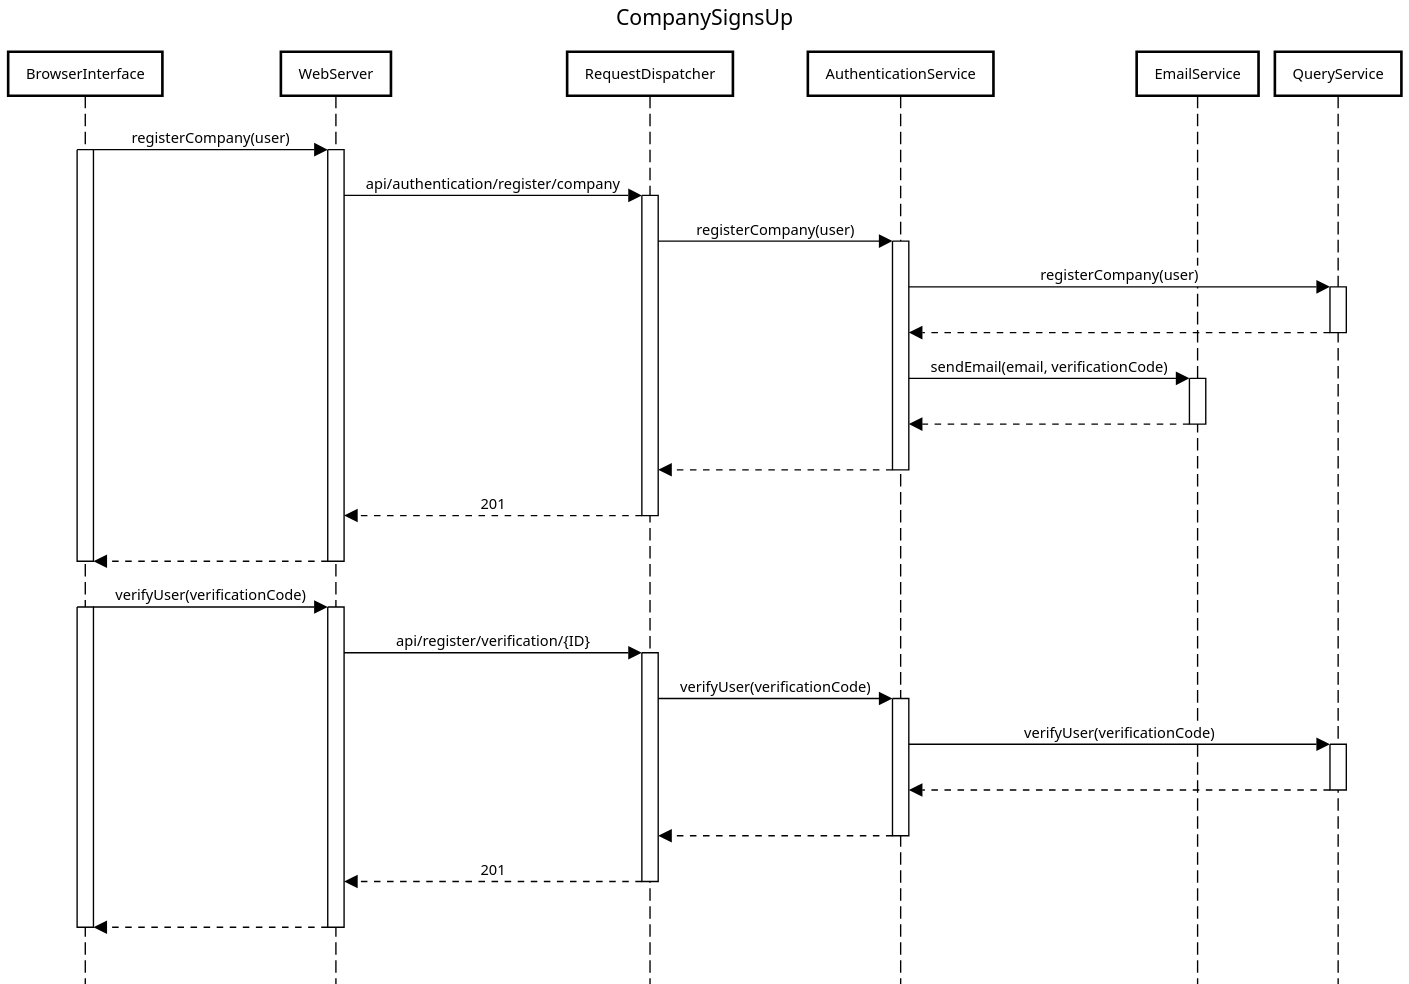
\includegraphics[width=0.8\linewidth]{../assets/runtime-views/CompanySignsUp.png}
    }
\end{figure}

\item \subsubsection{UserLogsIn}

To log in into the system, the user has to fill in the credentials fields and submit it.
This process is the same for both students and companies.
The whole process is handled by the authentication service component, that interacts with the query service to validate the information.
Once the user is logged in, the authentication service will generate a token, which is sent to the user.
With the token, the user can access the other website pages reserved for logged users.

\begin{figure}[H]
    \centering
    \fcolorbox{black}{white}{
        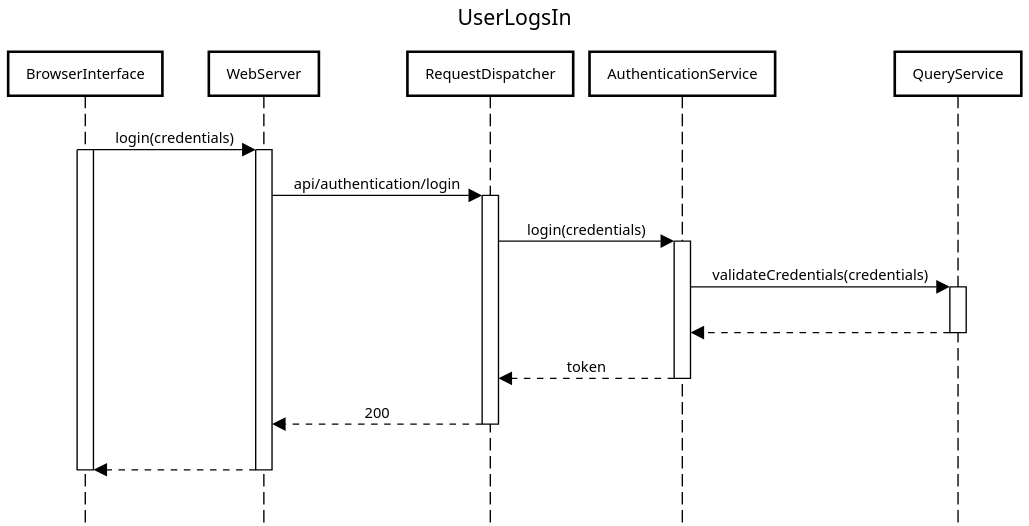
\includegraphics[width=0.8\linewidth]{../assets/runtime-views/UserLogsIn.png}
    }
\end{figure}

\item \subsubsection{StudentUploadsCV}

To upload the CV, the student is before hand authenticated by means of the token found in the header of the request.
Then, via the profile manager component, the CV is accepted, validated, and inserted into the file storage of the system.
The suggestion service is called afterwards, and if valid suggestions are found for the CV, they are notified to the student.

\begin{figure}[H]
    \centering
    \fcolorbox{black}{white}{
        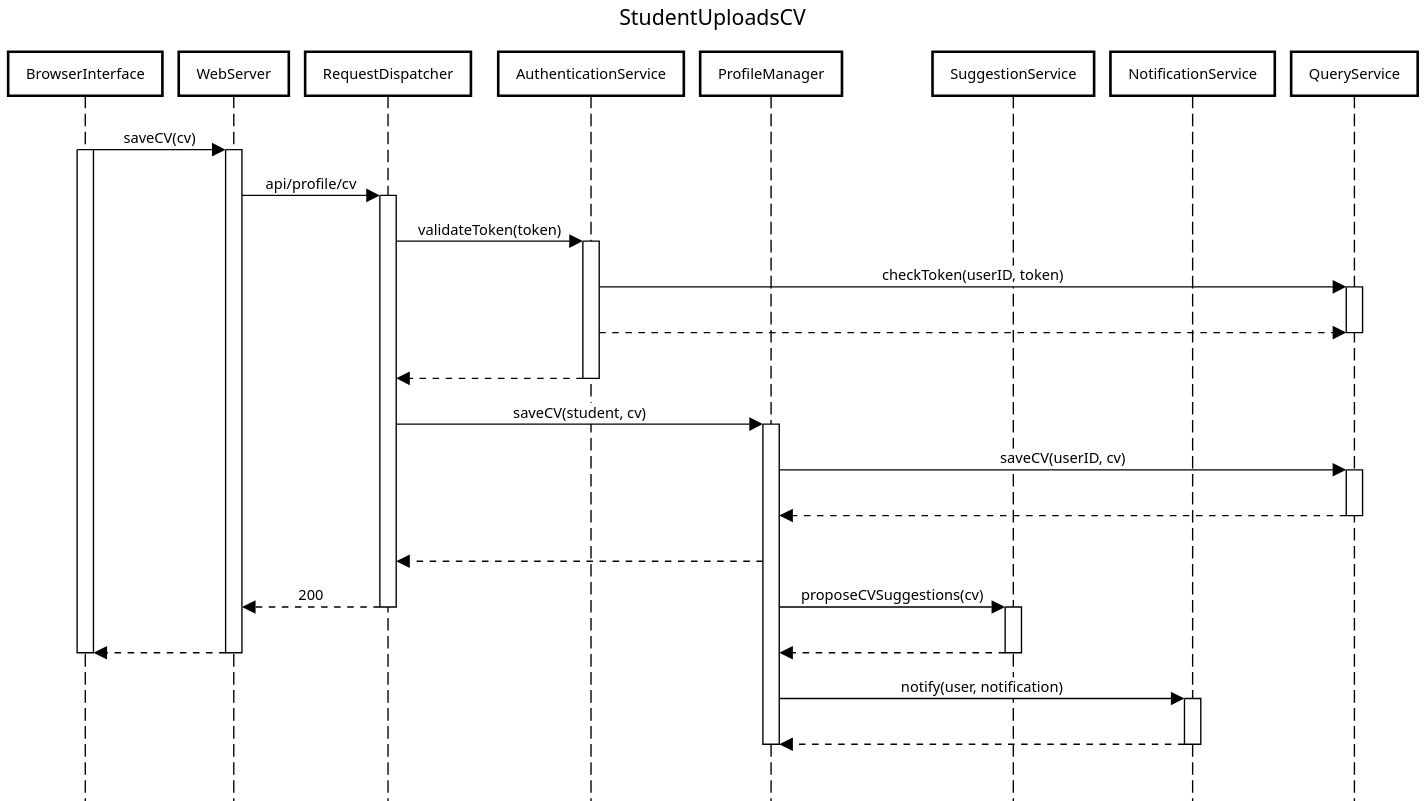
\includegraphics[width=0.8\linewidth]{../assets/runtime-views/StudentUploadsCV.png}
    }
\end{figure}

\item \subsubsection{CompanyCreatesAdvertisement}

To create an advertisement, the company is before hand authenticated by means of the token found in the header of the request.
Then, via the profile manager component, the advertisement is accepted, validated, and inserted into the DB.
The suggestion service is called afterwards, and if valid suggestions are found for the advertisement, they are notified to the company.

\begin{figure}[H]
    \centering
    \fcolorbox{black}{white}{
        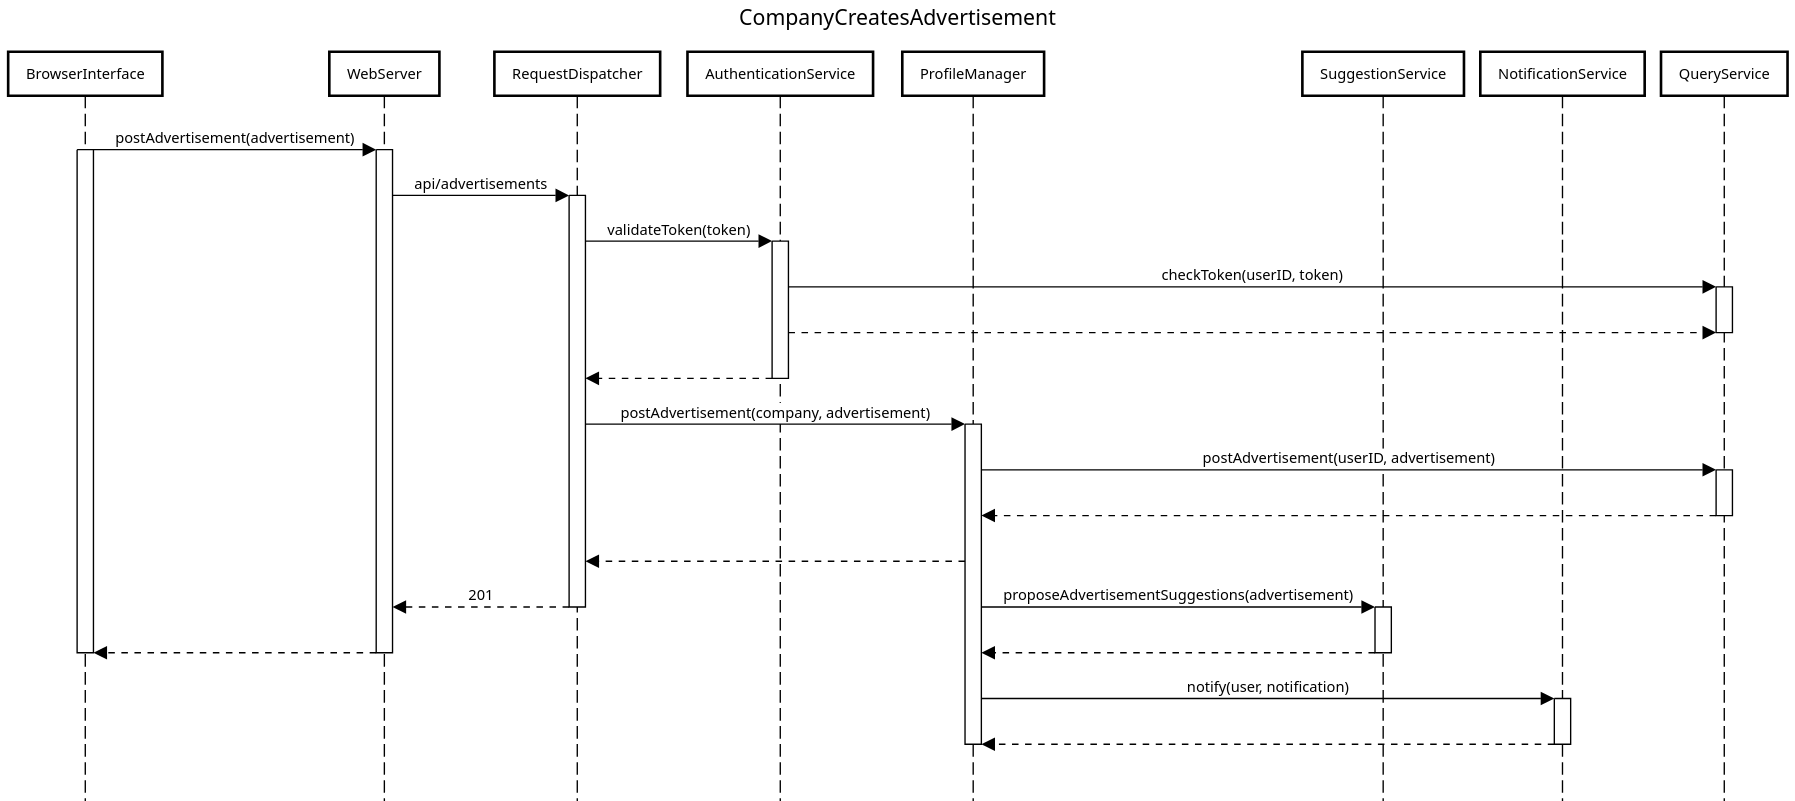
\includegraphics[width=0.8\linewidth]{../assets/runtime-views/CompanyCreatesAdvertisement.png}
    }
\end{figure}

\item \subsubsection{StudentVisualizesAdvertisements}

To visualize advertisements in the feed page, the student is before hand authenticated by means of the token found in the header of the request.
Then, the recommendation service uses keywords found in the student profile to find matching advertisements in the DB.
Those are returned to the student, which finds the feed page populated with the advertisements.

\begin{figure}[H]
    \centering
    \fcolorbox{black}{white}{
        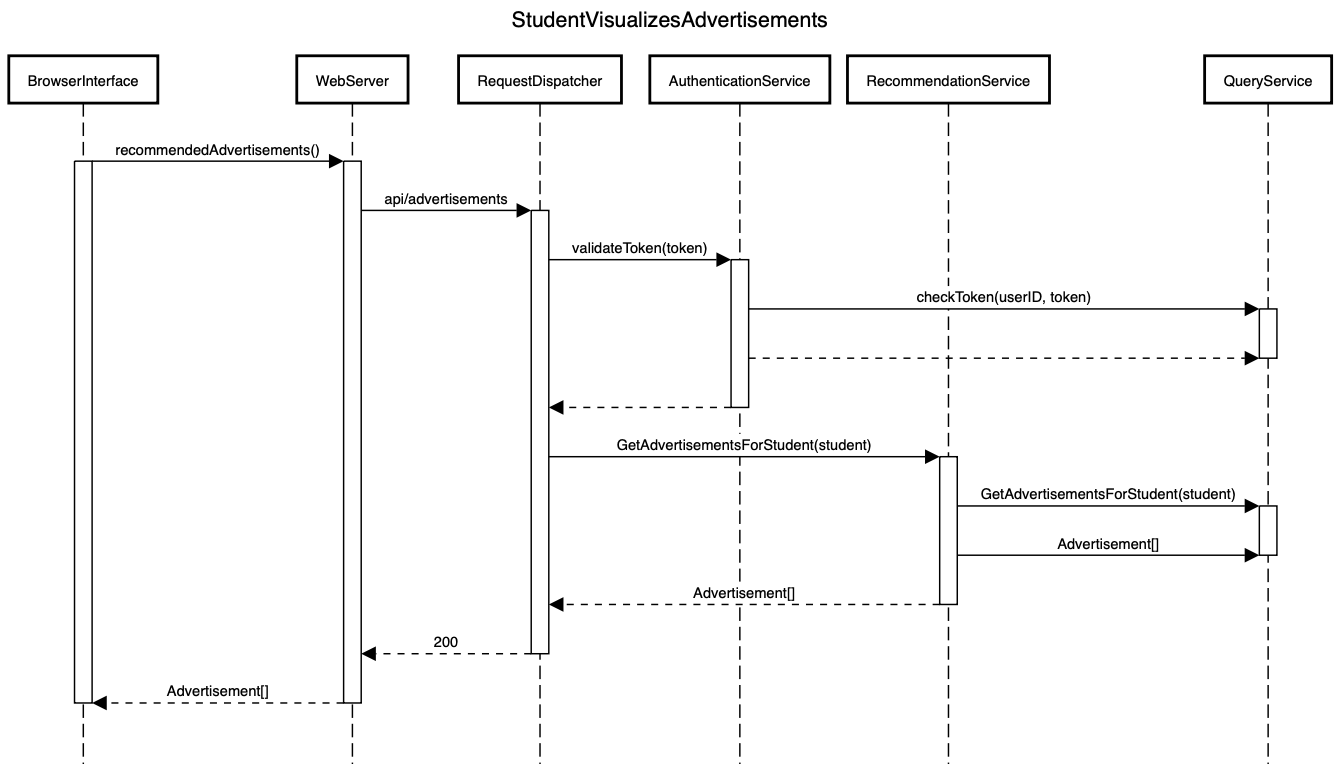
\includegraphics[width=0.8\linewidth]{../assets/runtime-views/StudentVisualizesAdvertisements.png}
    }
\end{figure}

\item \subsubsection{CompanyVisualizesCandidates}

To visualize eligible students in the feed page, the company is before hand authenticated by means of the token found in the header of the request.
Then, the recommendation service uses keywords found in the company profile and in the selected advertisement to find matching student candidates in the DB.
Those are returned to the company, which finds the feed page populated with the students information.

\begin{figure}[H]
    \centering
    \fcolorbox{black}{white}{
        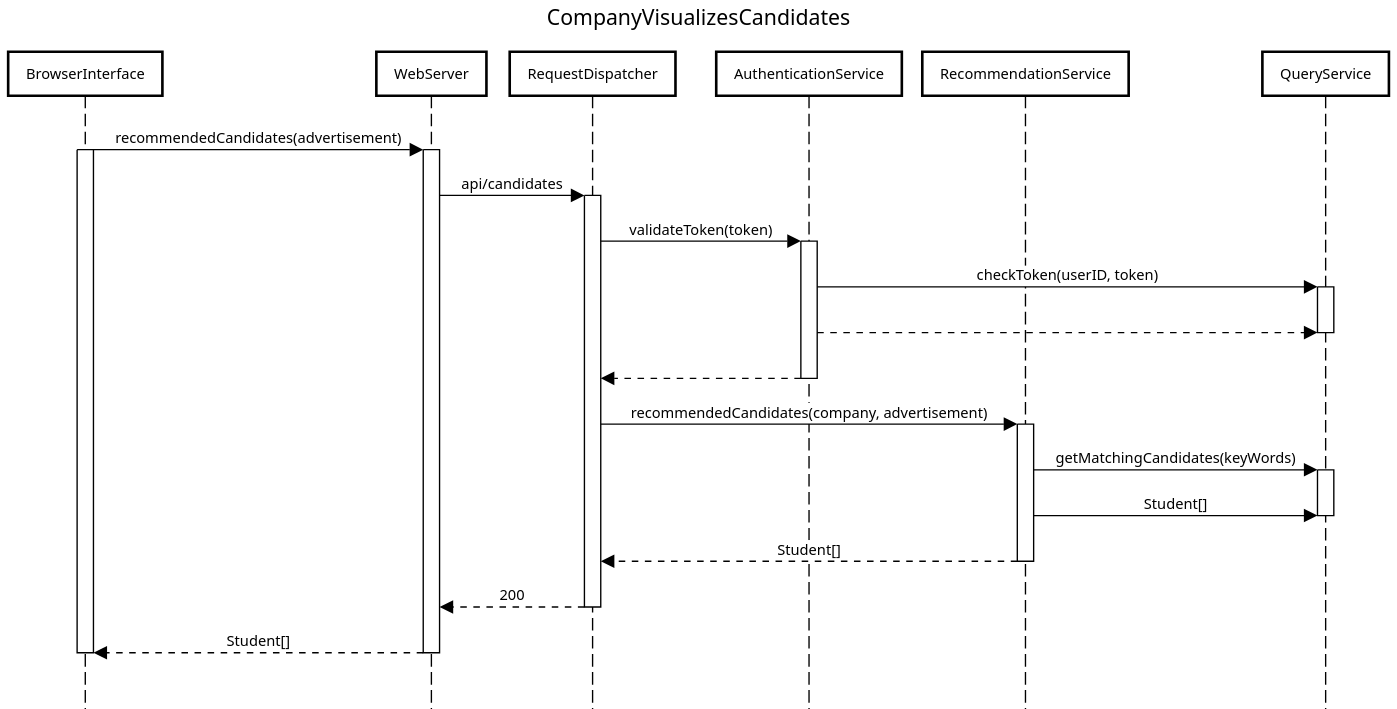
\includegraphics[width=0.8\linewidth]{../assets/runtime-views/CompanyVisualizesCandidates.png}
    }
\end{figure}

\item \subsubsection{CompanyCreatesQuestionnaire}

To build a new questionnaire, the company is before hand authenticated by means of the token found in the header of the request.
Then, via the enrollment manager component, the new questionnaire is accepted, validated, and inserted into the DB.

\begin{figure}[H]
    \centering
    \fcolorbox{black}{white}{
        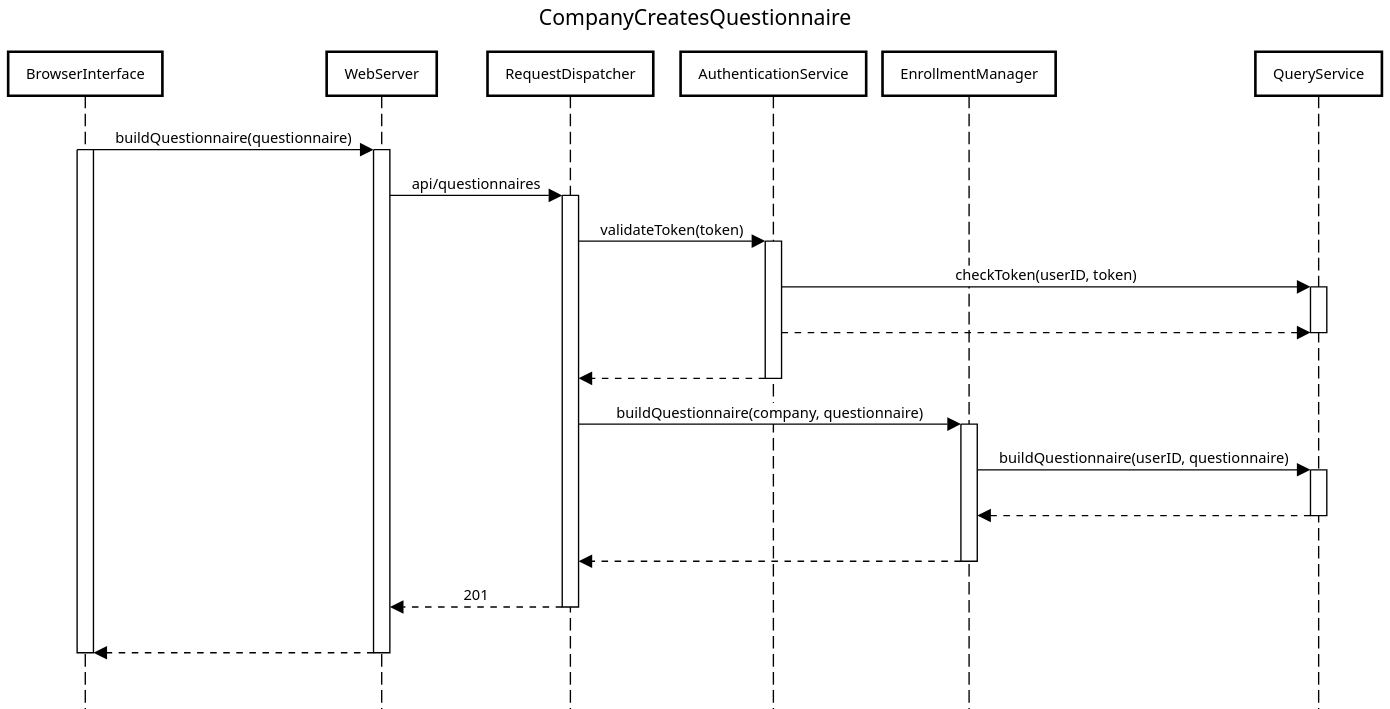
\includegraphics[width=0.8\linewidth]{../assets/runtime-views/CompanyCreatesQuestionnaire.png}
    }
\end{figure}

\item \subsubsection{StudentFillsQuestionnaire}

To fill in a questionnaire, the student is before hand authenticated by means of the token found in the header of the request.
Then, via the enrollment manager component, the filled in questionnaire is accepted, validated, and inserted into the DB.

\begin{figure}[H]
    \centering
    \fcolorbox{black}{white}{
        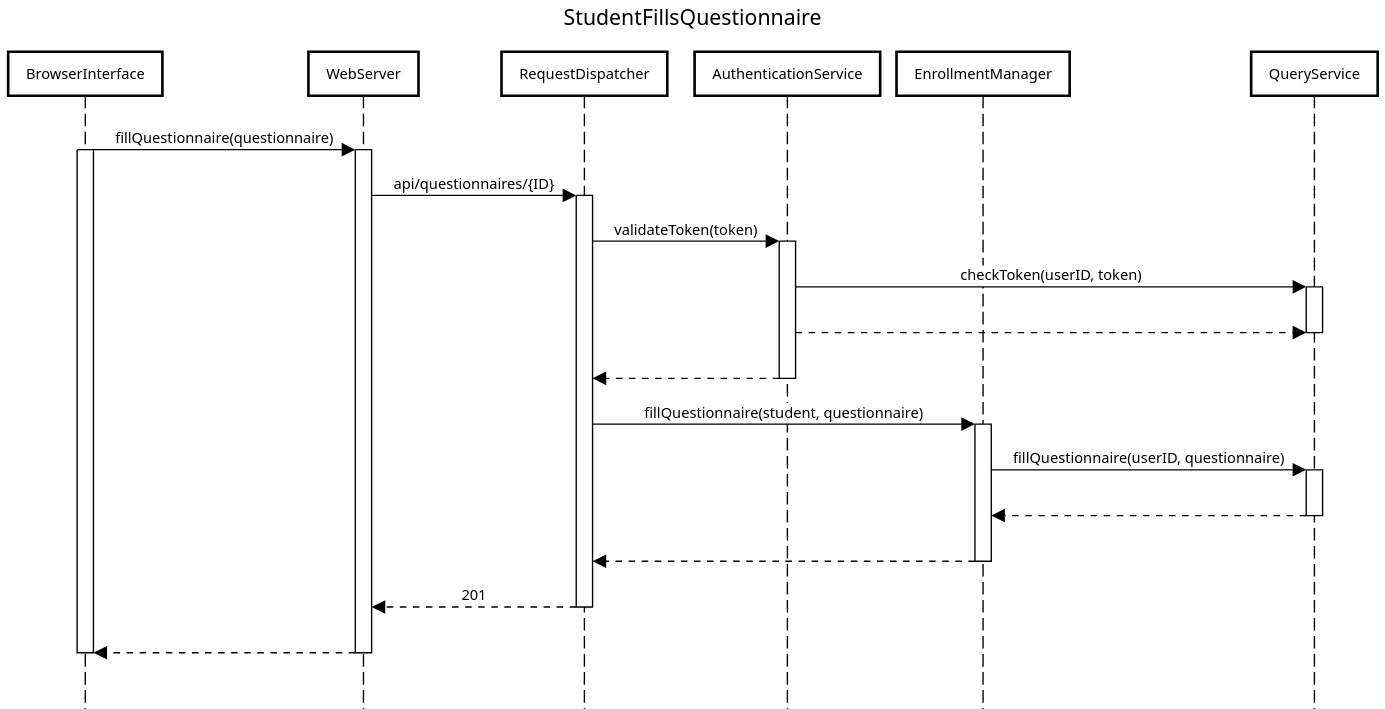
\includegraphics[width=0.8\linewidth]{../assets/runtime-views/StudentFillsQuestionnaire.png}
    }
\end{figure}

\item \subsubsection{CompanyAcceptsStudentEnrollment}

To accept the enrollment request made by a user, the company is before hand authenticated by means of the token found in the header of the request.
Then, via the enrollment manager component, the internship application, relative to a specific advertisement, is accepted, validated, and inserted into the DB.

\begin{figure}[H]
    \centering
    \fcolorbox{black}{white}{
        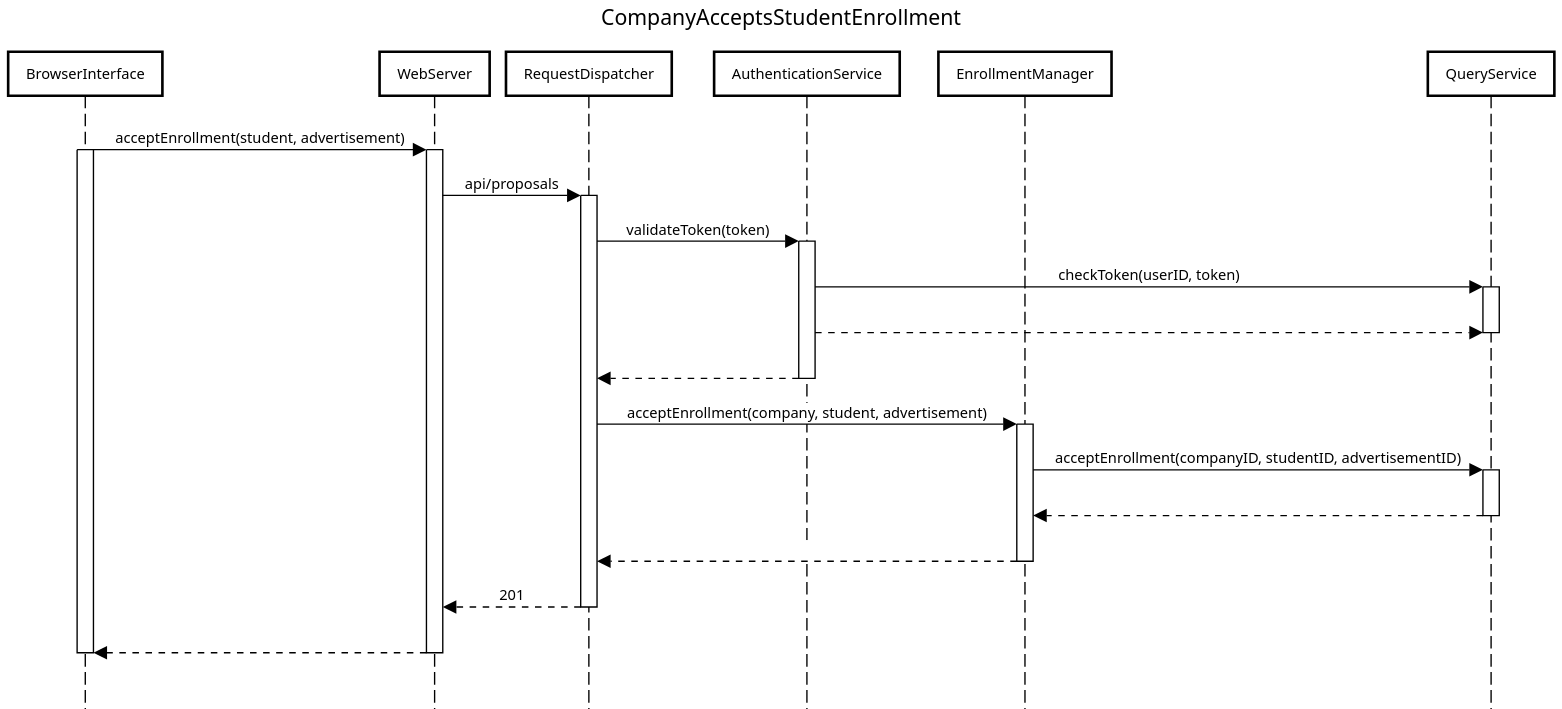
\includegraphics[width=0.8\linewidth]{../assets/runtime-views/CompanyAcceptsStudentEnrollment.png}
    }
\end{figure}

\item \subsubsection{StudentVisualizesInternshipInformation}

To visualize information about its ongoing internship, the student is before hand authenticated by means of the token found in the header of the request.
Then, via the internship manager component, the information about the internship is queried and returned to the student.

\begin{figure}[H]
    \centering
    \fcolorbox{black}{white}{
        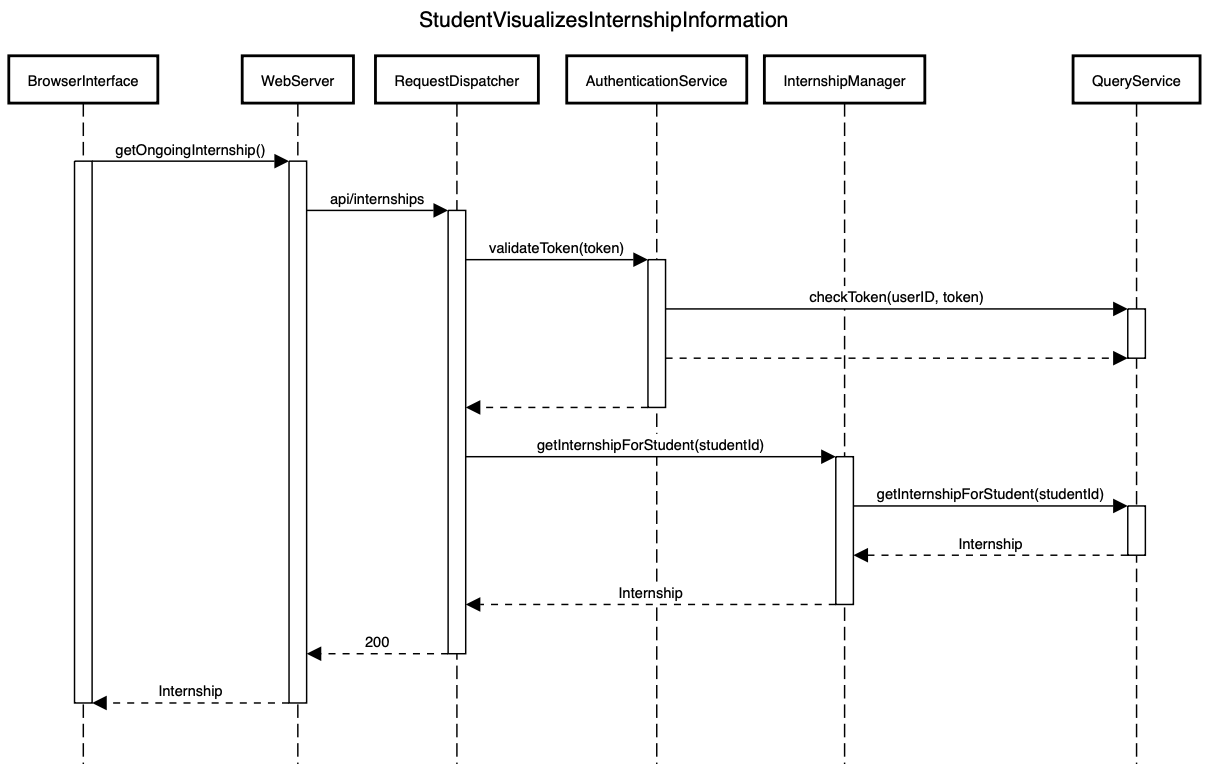
\includegraphics[width=0.8\linewidth]{../assets/runtime-views/StudentVisualizesInternshipInformation.png}
    }
\end{figure}

\item \subsubsection{CompanyVisualizesInternshipsInformation}

To visualize information about its ongoing internships, the company is before hand authenticated by means of the token found in the header of the request.
Then, via the internship manager component, the information about the internships is queried and returned to the company.

\begin{figure}[H]
    \centering
    \fcolorbox{black}{white}{
        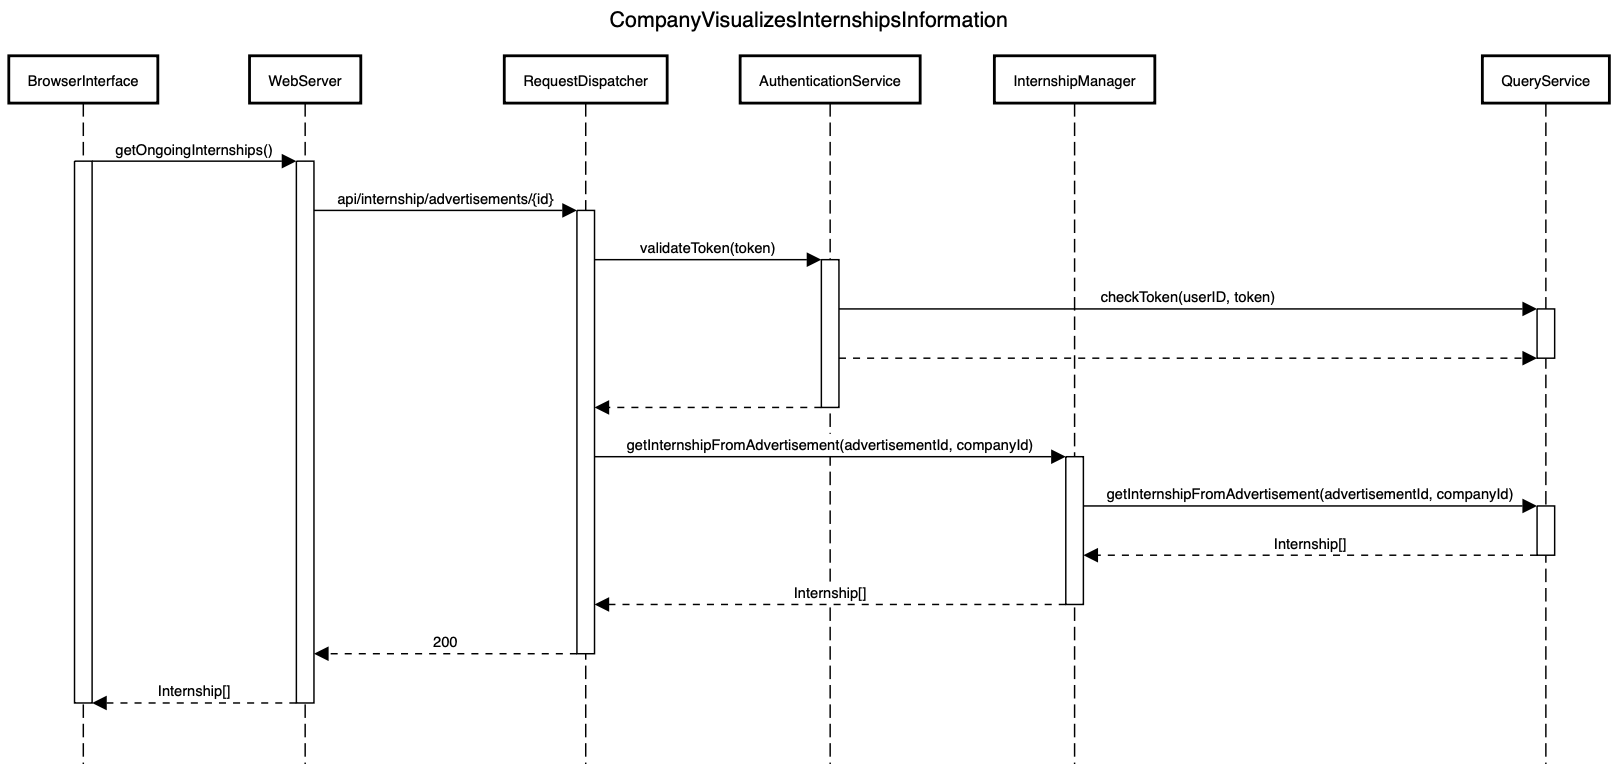
\includegraphics[width=0.8\linewidth]{../assets/runtime-views/CompanyVisualizesInternshipsInformation.png}
    }
\end{figure}

\item \subsubsection{UserSendsComplaint}

To send a complaint relative to an ongoing internship, the participant is before hand authenticated by means of the token found in the header of the request.
Then, via the internship manager and the complaint manager components, the complaint is accepted, validated and inserted into the DB.
The university will then be notified.

\begin{figure}[H]
    \centering
    \fcolorbox{black}{white}{
        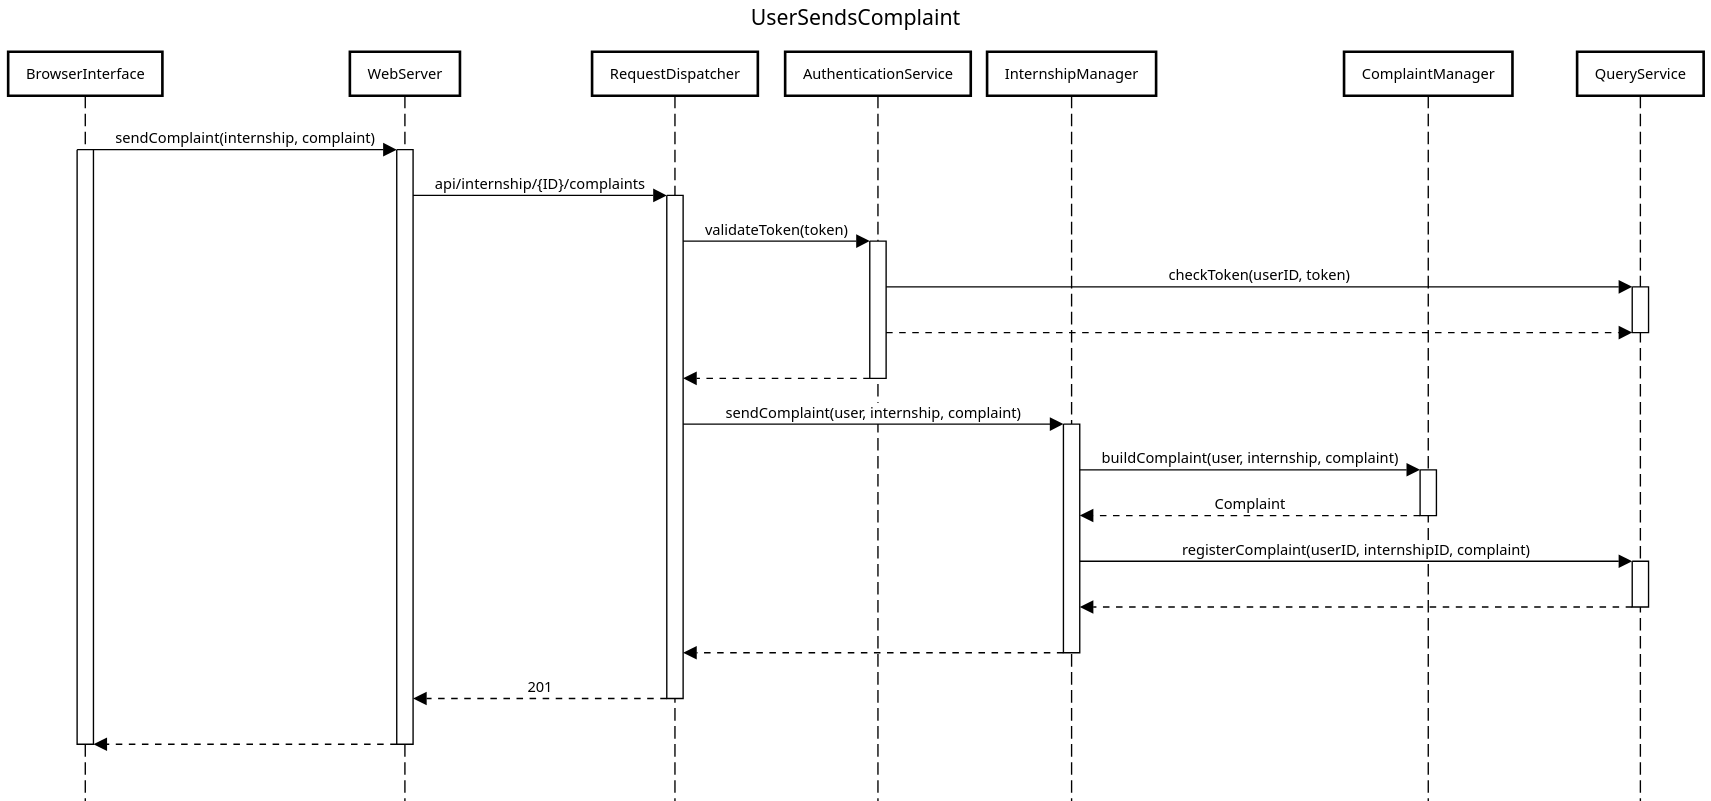
\includegraphics[width=0.8\linewidth]{../assets/runtime-views/UserSendsComplaint.png}
    }
\end{figure}

\item \subsubsection{UniversityVisualizesComplaints}

To visualize the complaints, the university is before hand authenticated by means of the token found in the header of the request.
Then, via the internship manager and complaint manager components, the complaints relative to its students internships are queried from the DB.
Those are returned to the university, which finds the complaints page populated with the complaints messages.

\begin{figure}[H]
    \centering
    \fcolorbox{black}{white}{
        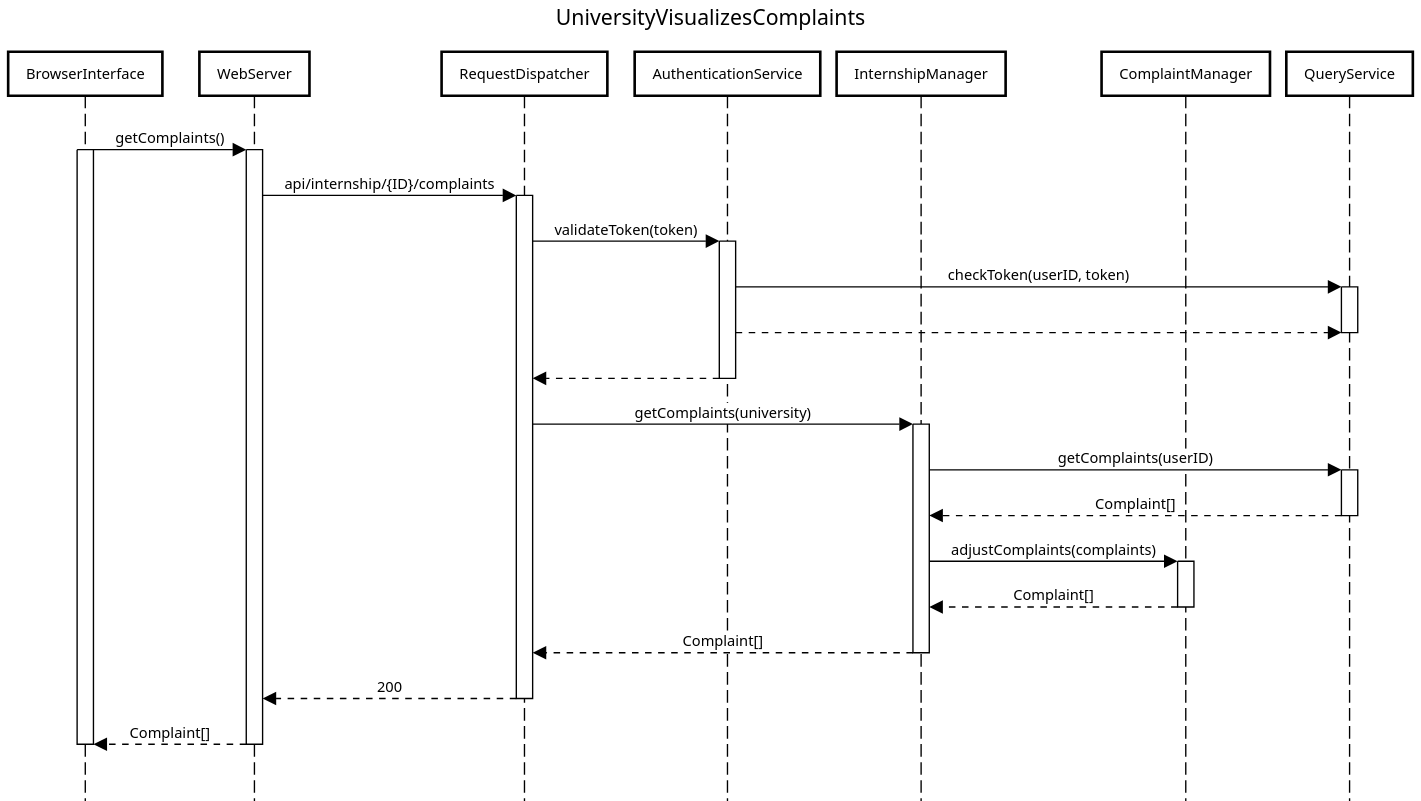
\includegraphics[width=0.8\linewidth]{../assets/runtime-views/UniversityVisualizesComplaints.png}
    }
\end{figure}

\item \subsubsection{UniversityEndsInternship}

To end an internship, the university is before hand authenticated by means of the token found in the header of the request.
Then, via the internship manager and complaint manager components, the internship of its student can be interrupted, if complaints have arose.
If that is the case, the DB is updated accordingly.

\begin{figure}[H]
    \centering
    \fcolorbox{black}{white}{
        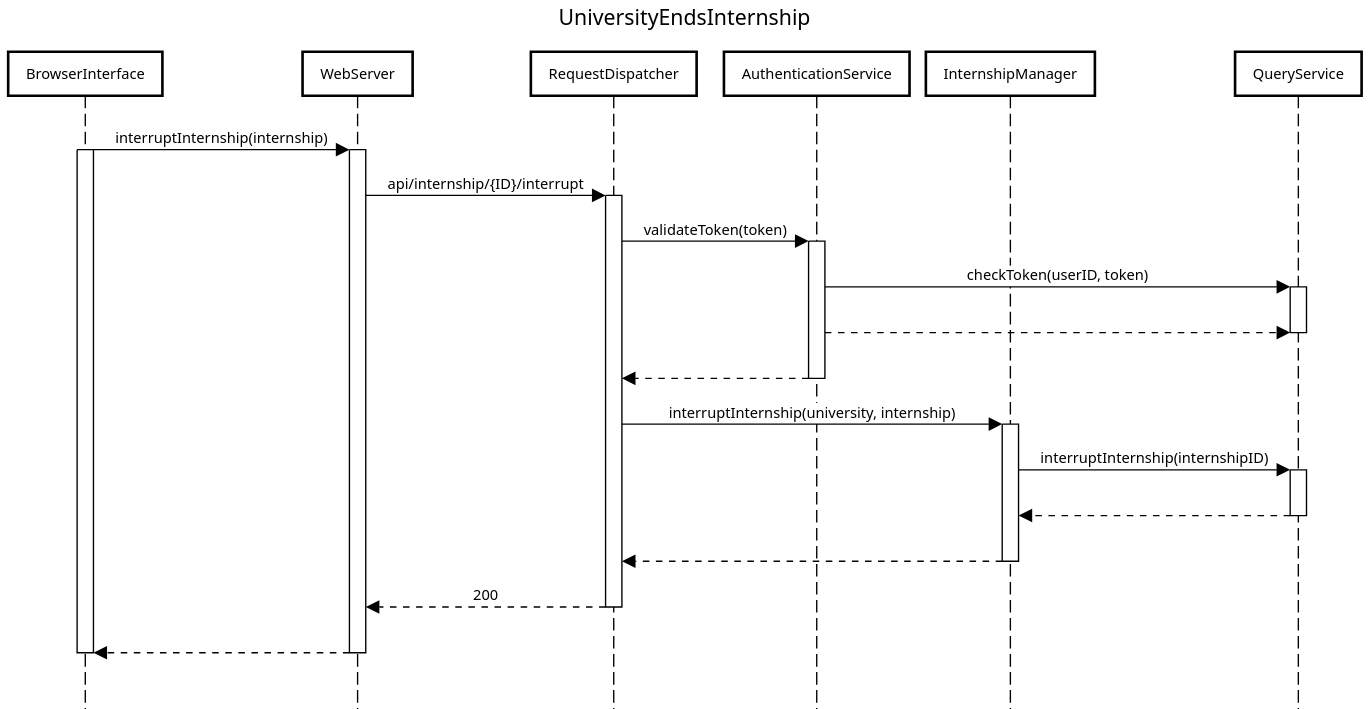
\includegraphics[width=0.8\linewidth]{../assets/runtime-views/UniversityEndsInternship.png}
    }
\end{figure}

\item \subsubsection{StudentFillsFeedbackForm}

To provide a feedback about a finished internship, the student is before hand authenticated by means of the token found in the header of the request.
Then, via the internship manager and the feedback manager components, the feedback form is accepted, validated and inserted into the DB.

\begin{figure}[H]
    \centering
    \fcolorbox{black}{white}{
        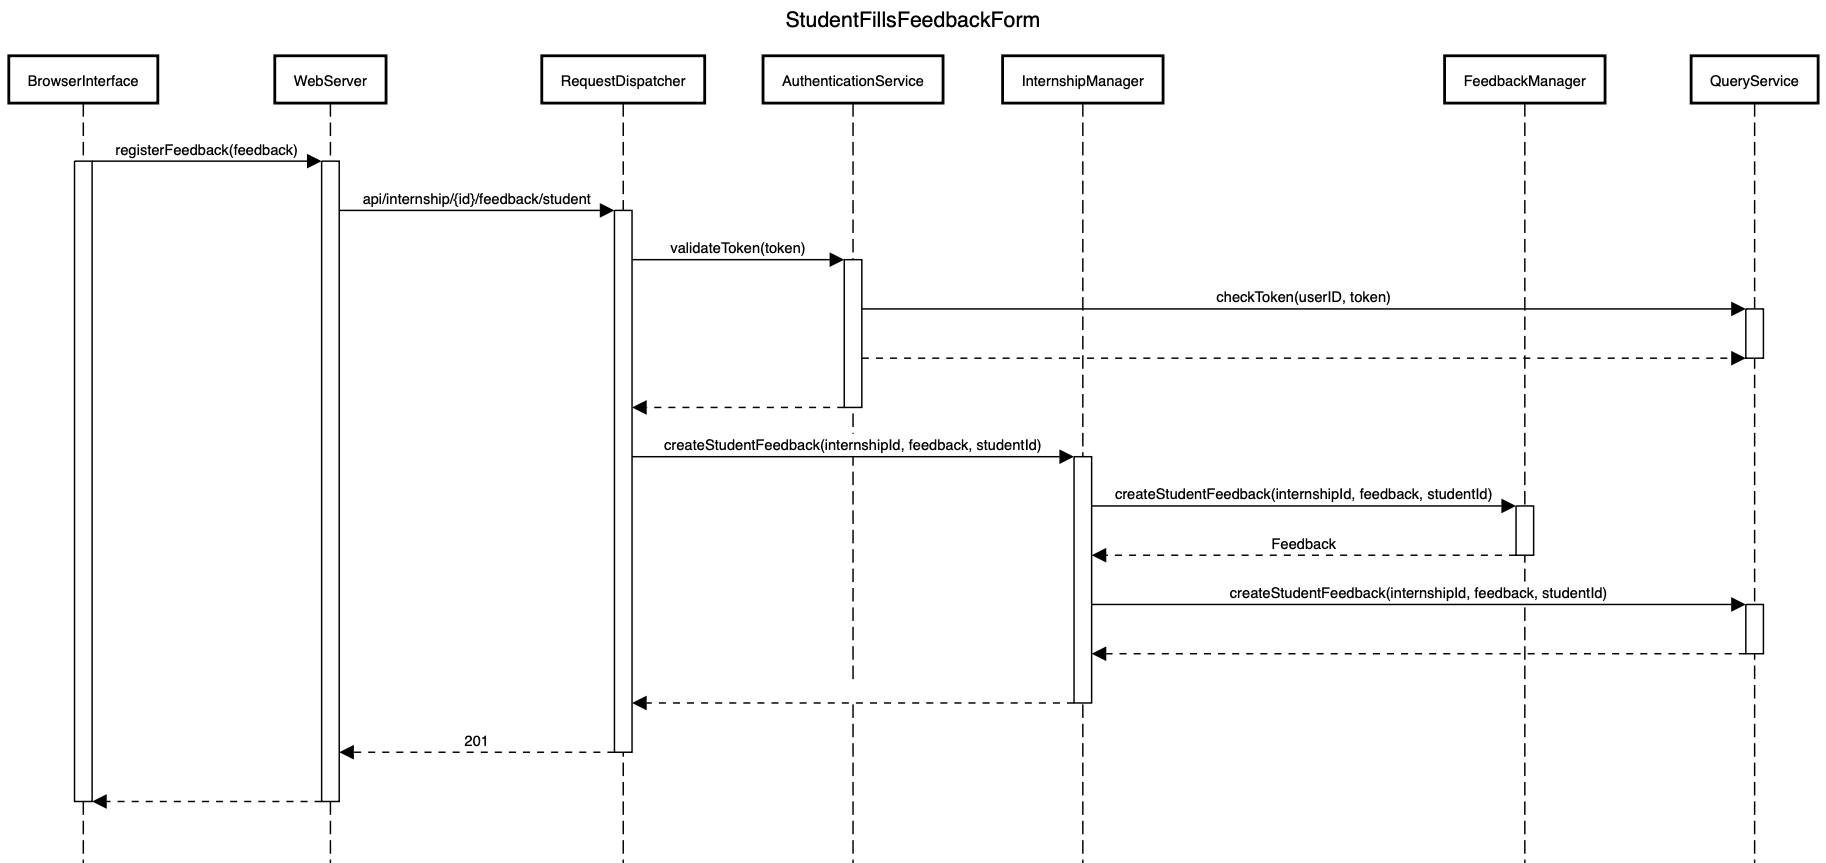
\includegraphics[width=0.8\linewidth]{../assets/runtime-views/StudentFillsFeedbackForm.png}
    }
\end{figure}

\item \subsubsection{CompanyFillsFeedbackForm}

To provide a feedback about a finished internship, the company is before hand authenticated by means of the token found in the header of the request.
Then, via the internship manager and the feedback manager components, the feedback form is accepted, validated and inserted into the DB.

\begin{figure}[H]
    \centering
    \fcolorbox{black}{white}{
        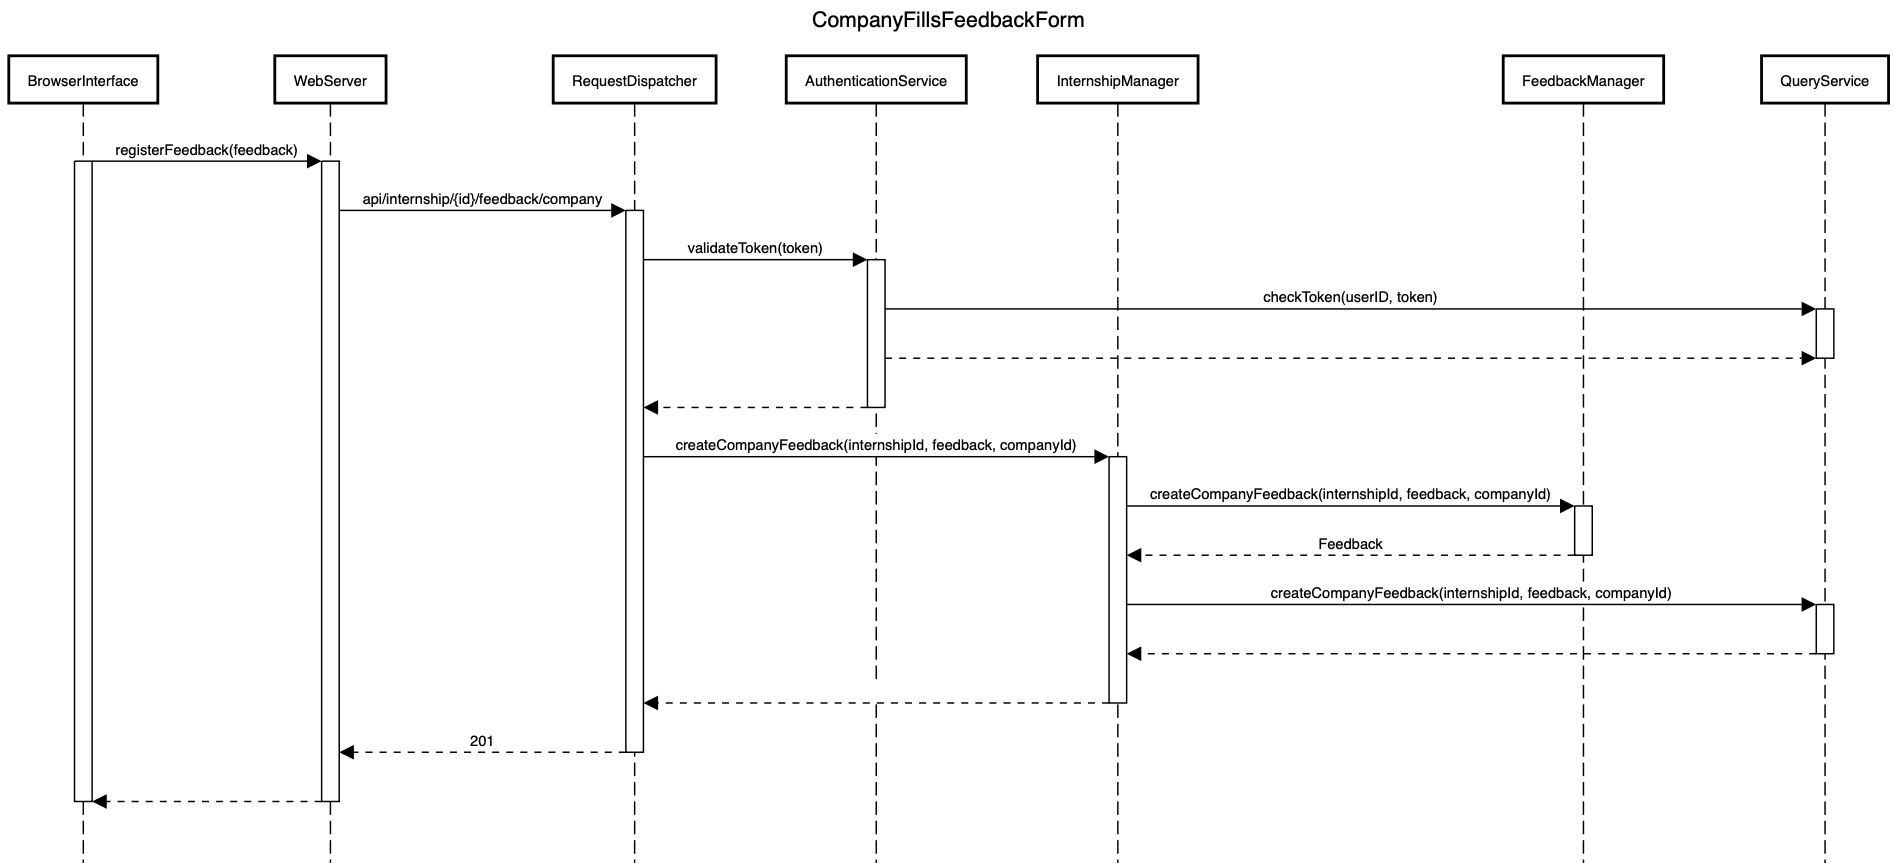
\includegraphics[width=0.8\linewidth]{../assets/runtime-views/CompanyFillsFeedbackForm.png}
    }
\end{figure}

\end{enumerate}

\section{Component interfaces}

\subsection{Application APIs}

\subsubsection{POST /api/authentication/register/company}
\begin{itemize}
    \item Description: register a company
    \item Request body: \verb|RegistrationFormCompany|
    \item Response 200: OK
    \item Response 400: Bad Request
    \item Response 500: Internal Server Error
\end{itemize}

\subsubsection{POST /api/authentication/register/student}
\begin{itemize}
    \item Description: register a student
    \item Request body: \verb|RegistrationFormStudent|
    \item Response 200: OK
    \item Response 400: Bad Request
    \item Response 500: Internal Server Error
\end{itemize}

\subsubsection{POST /api/authentication/login}
\begin{itemize}
    \item Description: log in a user from credentials
    \item Request body: \verb|Credentials|
    \item Response 200: OK
    \item Response 400: Bad Request
    \item Response 401: Unauthorized
\end{itemize}

\subsubsection{GET /api/authentication}
\begin{itemize}
    \item Description: check log in token validity
    \item Response 200: OK
    \item Response 401: Unauthorized
\end{itemize}

\subsubsection{POST /api/enrollment/applications/\{id\}}
\begin{itemize}
    \item Description: make an application request
    \item Request body: \verb|ApplicationRegistration|
    \item Response 200: OK
    \item Response 400: Bad Request
    \item Response 500: Internal Server Error
\end{itemize}

\subsubsection{GET /api/enrollment/applications/\{id\}}
\begin{itemize}
    \item Description: get pending applications
    \item Response 200: OK
    \item Response 400: Bad Request
    \item Response 404: Not Found
    \item Response 500: Internal Server Error
\end{itemize}

\subsubsection{POST /api/enrollment/accept/\{id\}}
\begin{itemize}
    \item Description: accept an application
    \item Request body: \verb|Date|
    \item Response 200: OK
    \item Response 400: Bad Request
    \item Response 404: Not Found
    \item Response 500: Internal Server Error
\end{itemize}

\subsubsection{POST /api/enrollment/reject/\{id\}}
\begin{itemize}
    \item Description: reject an application
    \item Response 200: OK
    \item Response 400: Bad Request
    \item Response 404: Not Found
    \item Response 500: Internal Server Error
\end{itemize}

\subsubsection{GET /api/internship}
\begin{itemize}
    \item Description: get internships for a student
    \item Response 200: OK
    \item Response 400: Bad Request
    \item Response 404: Not Found
\end{itemize}

\subsubsection{POST /api/internship/\{id\}/feedback/student}
\begin{itemize}
    \item Description: create feedback for a student
    \item Request body: \verb|Feedback|
    \item Response 200: OK
    \item Response 400: Bad Request
\end{itemize}

\subsubsection{GET /api/internship/\{id\}/feedback/student}
\begin{itemize}
    \item Description: get the student feedback
    \item Response 200: OK
    \item Response 400: Bad Request
\end{itemize}

\subsubsection{POST /api/internship/\{id\}/feedback/company}
\begin{itemize}
    \item Description: create feedback for a company
    \item Request body: \verb|Feedback|
    \item Response 200: OK
    \item Response 400: Bad Request
\end{itemize}

\subsubsection{GET /api/internship/\{id\}/feedback/company}
\begin{itemize}
    \item Description: get the company feedback
    \item Response 200: OK
    \item Response 400: Bad Request
\end{itemize}

\subsubsection{GET /api/internship/advertisements/\{id\}}
\begin{itemize}
    \item Description: get internships from an advertisement
    \item Response 200: OK
    \item Response 400: Bad Request
\end{itemize}

\subsubsection{POST /api/internship/delete/\{id\}}
\begin{itemize}
    \item Description: only for test, don't use
    \item Response 200: OK
    \item Response 404: Not Found
\end{itemize}

\subsubsection{POST /api/internship/delete/feedback/\{id\}}
\begin{itemize}
    \item Description: delete your feedback for the internship
    \item Response 200: OK
    \item Response 404: Not Found
\end{itemize}

\subsubsection{GET /api/notification}
\begin{itemize}
    \item Description: get notifications for a student
    \item Response 200: OK
    \item Response 400: Bad Request
    \item Response 404: Not Found
    \item Response 500: Internal Server Error
\end{itemize}

\subsubsection{POST /api/notification/delete/\{id\}}
\begin{itemize}
    \item Description: delete a notification for a student
    \item Response 200: OK
    \item Response 400: Bad Request
    \item Response 404: Not Found
\end{itemize}

\subsubsection{GET /api/profile/company}
\begin{itemize}
    \item Description: get the company profile information
    \item Response 200: OK
    \item Response 400: Bad Request
    \item Response 404: Not Found
\end{itemize}

\subsubsection{POST /api/profile/company}
\begin{itemize}
    \item Description: update the profile information of the company
    \item Request body: \verb|ProfileUpdateCompany|
    \item Response 200: OK
    \item Response 400: Bad Request
    \item Response 500: Internal Server Error
\end{itemize}

\subsubsection{GET /api/profile/student}
\begin{itemize}
    \item Description: get the student profile information
    \item Response 200: OK
    \item Response 400: Bad Request
    \item Response 500: Internal Server Error
\end{itemize}

\subsubsection{POST /api/profile/student}
\begin{itemize}
    \item Description: update the profile information of the student
    \item Request body: \verb|ProfileUpdateStudent|
    \item Response 200: OK
    \item Response 400: Bad Request
    \item Response 500: Internal Server Error
\end{itemize}

\subsubsection{GET /api/profile/company/\{id\}}
\begin{itemize}
    \item Description: get a company profile information
    \item Response 200: OK
    \item Response 400: Bad Request
    \item Response 404: Not Found
\end{itemize}

\subsubsection{GET /api/profile/student/\{id\}}
\begin{itemize}
    \item Description: get a student profile information
    \item Response 200: OK
    \item Response 400: Bad Request
    \item Response 404: Not Found
\end{itemize}

\subsubsection{GET /api/profile/cv}
\begin{itemize}
    \item Description: download the CV of the student
    \item Response 200: OK
    \item Response 404: Not Found
\end{itemize}

\subsubsection{POST /api/profile/cv}
\begin{itemize}
    \item Description: upload the CV of a student
    \item Request body: \verb|CV|
    \item Response 200: OK
    \item Response 400: Bad Request
    \item Response 500: Internal Server Error
\end{itemize}

\subsubsection{GET /api/profile/cv/\{id\}}
\begin{itemize}
    \item Description: download the CV of a student
    \item Response 200: OK
    \item Response 400: Bad Request
    \item Response 404: Not Found
\end{itemize}

\subsubsection{POST /api/profile/cv/delete}
\begin{itemize}
    \item Description: delete the CV of a student
    \item Response 200: OK
    \item Response 404: Not Found
\end{itemize}

\subsubsection{POST /api/profile/delete}
\begin{itemize}
    \item Description: delete the user
    \item Response 200: OK
    \item Response 404: Not Found
\end{itemize}

\subsubsection{POST /api/profile/skills}
\begin{itemize}
    \item Description: add a skill into the student profile
    \item Request body: \verb|SkillRegistration|
    \item Response 200: OK
    \item Response 400: Bad Request
    \item Response 500: Internal Server Error
\end{itemize}

\subsubsection{GET /api/profile/skills}
\begin{itemize}
    \item Description: get the skills of the student
    \item Response 200: OK
    \item Response 400: Bad Request
    \item Response 404: Not Found
    \item Response 500: Internal Server Error
\end{itemize}

\subsubsection{GET /api/profile/skills/\{id\}}
\begin{itemize}
    \item Description: get the skills of a student
    \item Response 200: OK
    \item Response 400: Bad Request
    \item Response 404: Not Found
    \item Response 500: Internal Server Error
\end{itemize}

\subsubsection{POST /api/profile/skills/delete/\{id\}}
\begin{itemize}
    \item Description: delete a skill from profile
    \item Response 200: OK
    \item Response 400: Bad Request
    \item Response 404: Not Found
\end{itemize}

\subsubsection{GET /api/recommendation/advertisements}
\begin{itemize}
    \item Description: get distinct advertisements for a student or for a company
    \item Response 200: OK
    \item Response 400: Bad Request
    \item Response 500: Internal Server Error
\end{itemize}

\subsubsection{POST /api/recommendation/advertisements}
\begin{itemize}
    \item Description: create a new advertisement
    \item Request body: \verb|AdvertisementRegistration|
    \item Response 200: OK
    \item Response 400: Bad Request
    \item Response 500: Internal Server Error
\end{itemize}

\subsubsection{GET /api/recommendation/advertisements/\{id\}}
\begin{itemize}
    \item Description: get a specific advertisement
    \item Response 200: OK
    \item Response 400: Bad Request
    \item Response 404: Not Found
\end{itemize}

\subsubsection{GET /api/recommendation/candidates/advertisements/\{id\}}
\begin{itemize}
    \item Description: get recommended students for specific advertisements
    \item Response 200: OK
    \item Response 400: Bad Request
\end{itemize}

\subsubsection{POST /api/recommendation/suggestions/advertisement/\{id\}/student/\{id\}}
\begin{itemize}
    \item Description: create a new suggestion by a company for one student
    \item Response 200: OK
    \item Response 400: Bad Request
    \item Response 404: Not Found
\end{itemize}

\subsubsection{POST /api/recommendation/delete/\{id\}}
\begin{itemize}
    \item Description: delete an advertisement
    \item Response 200: OK
    \item Response 400: Bad Request
    \item Response 404: Not Found
\end{itemize}

\subsection{Interface methods}

\subsubsection{IEnrollmentQueries}
\begin{itemize}
    \item \verb|Entity.Application GetApplication(int userId, int advertisementId)|
    \item \verb|Entity.Application GetApplication(int applicationId)|
    \item \verb|bool CreateApplication(int userId, int advertisementId,| \\ \makebox[10em][l]{} \verb| string questionnaireAnswer)|
    \item \verb|List<Entity.Application> GetPendingApplications(int id)|
    \item \verb|bool AcceptApplication(int id)|
    \item \verb|bool RejectApplication(int id)|
    \item \verb|bool CreateInternship(int studentId, int companyId,| \\ \makebox[10em][l]{} \verb| int advertisementId, DateTime start, DateTime end)|
    \item \verb|bool NotifyStudent(int studentId, int advertisementId, bool accepted)|
    \item \verb|bool RejectAllApplications(int id)|
    \item \verb|bool UpdateAdvertisementSpots(int id)|
\end{itemize}

\subsubsection{IRecommendationQueries}
\begin{itemize}
    \item \verb|List<Entity.Advertisement> GetAdvertisementsOfCompany(int companyId)|
    \item \verb|List<Entity.Advertisement> GetAdvertisementsForStudent(int studentId)|
    \item \verb|int? CreateAdvertisement(int companyId,| \\ \makebox[10em][l]{} \verb| Entity.Advertisement advertisement, List<Entity.Skill> skills)|
    \item \verb|void MatchAdvertisementForStudent(int advertisementId)|
    \item \verb|Entity.Advertisement GetAdvertisement(int advertisementId)|
    \item \verb|List<Entity.Student> GetRecommendedCandidates(int companyId,| \\ \makebox[10em][l]{} \verb| int advertisementId)|
    \item \verb|bool CreateSuggestionsForStudent(int advertisementId, int studentId,| \\ \makebox[10em][l]{} \verb| int companyId)|
    \item \verb|bool DeleteAdvertisement(int advertisementId, int companyId)|
\end{itemize}

\subsubsection{IProfileService}
\begin{itemize}
    \item \verb|Company GetCompany(int id)|
    \item \verb|Student GetStudent(int id)|
    \item \verb|bool UpdateProfileCompany(int id, DTO.ProfileUpdateCompany updateForm)|
    \item \verb|bool UpdateProfileStudent(int id, DTO.ProfileUpdateStudent updateForm)|
    \item \verb|bool IsCompanyUpdateFormValid(DTO.ProfileUpdateCompany updateForm)|
    \item \verb|bool IsStudentUpdateFormValid(DTO.ProfileUpdateStudent updateForm)|
    \item \verb|bool CheckCvValidity(IFormFile file)|
    \item \verb|bool StoreCvFile(int id, IFormFile file)|
    \item \verb|IFormFile RetrieveCvFile(int id)|
    \item \verb|bool DeleteCv(int id)|
    \item \verb|bool DeleteUser(UserType type, int id)|
    \item \verb|bool AddSkill(int id, string name)|
    \item \verb|List<Skill> GetSkills(int id)|
    \item \verb|bool DeleteSkill(int skillId, int studentId)|
\end{itemize}

\subsubsection{IRecommendationService}
\begin{itemize}
    \item \verb|List<Advertisement> GetAdvertisementsOfCompany(int companyId)|
    \item \verb|List<Advertisement> GetAdvertisementsForStudent(int studentId)|
    \item \verb|bool CreateAdvertisement(int companyId,| \\ \makebox[10em][l]{} \verb| DTO.AdvertisementRegistration advertisement)|
    \item \verb|Advertisement GetAdvertisement(int advertisementId)|
    \item \verb|List<Student> GetRecommendedCandidates(int companyId, int advertisementId)|
    \item \verb|bool CreateSuggestionsForStudent(int advertisementId, int studentId,| \\ \makebox[10em][l]{} \verb| int companyId)|
    \item \verb|bool DeleteAdvertisement(int advertisementId, int companyId)|
\end{itemize}

\subsubsection{IAuthenticationQueries}
\begin{itemize}
    \item \verb|bool RegisterCompany(Entity.Company user)|
    \item \verb|bool RegisterStudent(Entity.Student user)|
    \item \verb|Entity.Company FindCompanyFromUsername(string username)|
    \item \verb|Entity.Student FindStudentFromUsername(string username)|
    \item \verb|Entity.Company FindCompanyFromEmail(string email)|
    \item \verb|Entity.Student FindStudentFromEmail(string email)|
\end{itemize}

\subsubsection{IFileService}
\begin{itemize}
    \item \verb|string GetCvFilePath(string fileName)|
    \item \verb|bool SaveFile(string filePath, byte[] fileData)|
    \item \verb|byte[] RetrieveFile(string filePath)|
    \item \verb|bool DeleteFile(string filePath)|
\end{itemize}

\subsubsection{IEnrollmentService}
\begin{itemize}
    \item \verb|Application GetApplication(int userId, int advertisementId)|
    \item \verb|Application GetApplication(int applicationId)|
    \item \verb|bool CreateApplication(int userId, int advertisementId,| \\ \makebox[10em][l]{} \verb| string questionnaireAnswer)|
    \item \verb|Advertisement GetAdvertisement(int id)|
    \item \verb|List<Application> GetPendingApplications(int id)|
    \item \verb|bool CheckStartDateValidity(DateTime date)|
    \item \verb|bool AcceptApplication(int id)|
    \item \verb|bool RejectApplication(int id)|
    \item \verb|bool CreateInternship(int studentId, int companyId,| \\ \makebox[10em][l]{} \verb| int advertisementId, DateTime start)|
    \item \verb|bool NotifyStudent(int studentId, int advertisementId, bool accepted)|
    \item \verb|Internship GetInternship(int id)|
    \item \verb|bool RejectAllApplications(int id)|
    \item \verb|bool UpdateAdvertisementSpots(int id)|
\end{itemize}

\subsubsection{IInternshipQueries}
\begin{itemize}
    \item \verb|Entity.Internship GetInternshipForStudent(int studentId)|
    \item \verb|List<Entity.Internship> GetInternshipFromAdvertisement(| \\ \makebox[10em][l]{} \verb|int advertisementId, int companyId)|
    \item \verb|bool CreateStudentFeedback(int internshipId,| \\ \makebox[10em][l]{} \verb| Entity.StudentFeedback feedback, int studentId)|
    \item \verb|bool CreateCompanyFeedback(int internshipId,| \\ \makebox[10em][l]{} \verb| Entity.CompanyFeedback feedback, int companyId)|
    \item \verb|Entity.StudentFeedback GetStudentFeedback(int internshipId,| \\ \makebox[10em][l]{} \verb| int userId, string role)|
    \item \verb|Entity.CompanyFeedback GetCompanyFeedback(int internshipId,| \\ \makebox[10em][l]{} \verb| int userId, string role)|
    \item \verb|bool DeleteInternship(int internshipId, int userId, string role)|
    \item \verb|bool DeleteStudentFeedback(int internshipId, int userId)|
    \item \verb|bool DeleteCompanyFeedback(int internshipId, int userId)|
\end{itemize}

\subsubsection{IDataService}
\begin{itemize}
    \item \verb|MySqlConnection GetConnection()|
    \item \verb|List<Entity.Student> MapToStudents(IDataReader reader)|
    \item \verb|List<Entity.Company> MapToCompanies(IDataReader reader)|
    \item \verb|List<Entity.Skill> MapToSkills(IDataReader reader)|
    \item \verb|List<Entity.Advertisement> MapToAdvertisements(IDataReader reader)|
    \item \verb|List<Entity.StudentNotifications> MapToStudentNotifications(| \\ \makebox[10em][l]{} \verb|IDataReader reader)|
    \item \verb|List<Entity.Application> MapToApplications(IDataReader reader)|
    \item \verb|List<Entity.Internship> MapToInternships(IDataReader reader)|
    \item \verb|List<Entity.StudentFeedback> MapToStudentFeedback(IDataReader reader)|
    \item \verb|List<Entity.CompanyFeedback> MapToCompanyFeedback(IDataReader reader)|
    \item \verb|List<string> MapToStrings(IDataReader reader, string fieldName)|
    \item \verb|List<int> MapToInts(IDataReader reader, string fieldName)|
\end{itemize}

\subsubsection{IInternshipService}
\begin{itemize}
    \item \verb|Internship GetInternshipForStudent(int studentId)|
    \item \verb|List<Internship> GetInternshipFromAdvertisement(int advertisementId,| \\ \makebox[10em][l]{} \verb| int companyId)|
    \item \verb|bool CreateStudentFeedback(int internshipId, DTO.Feedback feedback,| \\ \makebox[10em][l]{} \verb| int studentId)|
    \item \verb|bool CreateCompanyFeedback(int internshipId, DTO.Feedback feedback,| \\ \makebox[10em][l]{} \verb| int companyId)|
    \item \verb|DTO.Feedback GetStudentFeedback(int internshipId, int userId, string role)|
    \item \verb|DTO.Feedback GetCompanyFeedback(int internshipId, int userId, string role)|
    \item \verb|bool DeleteInternship(int internshipId, int userId, string role)|
    \item \verb|bool DeleteFeedback(int internshipId, int userId, string role)|
\end{itemize}

\subsubsection{INotificationService}
\begin{itemize}
    \item \verb|List<StudentNotifications> GetStudentNotifications(int studentId)|
    \item \verb|bool DeleteNotification(int notificationId, int studentId)|
\end{itemize}

\subsubsection{IAuthenticationService}
\begin{itemize}
    \item \verb|bool IsCompanyRegistrationValid(DTO.RegistrationFormCompany registrationForm)|
    \item \verb|bool IsStudentRegistrationValid(DTO.RegistrationFormStudent registrationForm)|
    \item \verb|bool RegisterCompany(DTO.RegistrationFormCompany registrationForm)|
    \item \verb|bool RegisterStudent(DTO.RegistrationFormStudent registrationForm)|
    \item \verb|User ValidateCredentials(DTO.Credentials credentials)|
    \item \verb|string GenerateToken(User user)|
    \item \verb|string HashPassword(string salt, string password)|
    \item \verb|string GenerateSalt()|
    \item \verb|bool IsValidEmail(string email)|
\end{itemize}

\subsubsection{INotificationQueries}
\begin{itemize}
    \item \verb|List<Entity.StudentNotifications> GetStudentNotifications(int studentId)|
    \item \verb|bool DeleteNotification(int notificationId, int studentId)|
\end{itemize}

\subsubsection{IProfileQueries}
\begin{itemize}
    \item \verb|Entity.Company FindCompanyFromId(int id)|
    \item \verb|Entity.Student FindStudentFromId(int id)|
    \item \verb|bool UpdateSaltAndPassword(UserType type, int id, string salt, string hash)|
    \item \verb|bool UpdateUsername(UserType type, int id, string username)|
    \item \verb|bool UpdateEmail(UserType type, int id, string email)|
    \item \verb|bool UpdateBio(UserType type, int id, string bio)|
    \item \verb|bool UpdateHeadquarter(int id, string headquarter)|
    \item \verb|bool UpdateFiscalCode(int id, string fiscalCode)|
    \item \verb|bool UpdateVatNumber(int id, string vatNumber)|
    \item \verb|bool UpdateName(int id, string name)|
    \item \verb|bool UpdateSurname(int id, string surname)|
    \item \verb|bool UpdateUniversity(int id, string university)|
    \item \verb|bool UpdateCourseOfStudy(int id, string courseOfStudy)|
    \item \verb|bool UpdateGender(int id, char gender)|
    \item \verb|bool UpdateBirthDate(int id, DateTime birthDate)|
    \item \verb|bool DeleteUser(UserType type, int id)|
    \item \verb|int FindSkill(string name)|
    \item \verb|bool AddSkill(string name)|
    \item \verb|bool AddSkillToStudent(int studentId, int skillId)|
    \item \verb|List<Entity.Skill> GetSkills(int id)|
    \item \verb|bool DeleteSkill(int skillId, int studentId)|
\end{itemize}

\section{Architectural styles and patterns}

\htitle{Three-tier architecture}
Since the S\&C platform is offered through the web, the client-server architecture is the most suitable for this kind of application.
In particular, a three-tier architecture comes handy when dividing the system into the three main logical layers: presentation (web server), business logic (application server), and data storage (database).
Each tier has its specific functions, ensuring separation of concerns and efficient management of the system.
It allows scalability, simplifies maintenance, and enhances control and security.

\htitle{REST}
The communication between the web server and the application server is based on the REST architectural style.
REST is stateless, meaning that the server does not need to store any information about the session, allowing higher scalability.
Moreover, it provides a uniform and easy interface via the HTTP methods (GET, POST, PUT, DELETE).

\htitle{MVC}
The MVC pattern is used to separate the presentation layer from the business logic.
In particular, the model contains the definitions of all the elements of the application, the view is the browser interface component, and the controller comprehends all the other application server services and managers.
This pattern allows a more maintainable application, since changes in one layer do not affect other layers.

\section{Other design decisions}

\htitle{Scale out}
Using a scale out design, when implementing the software, can highly enhance availability, by avoiding the need of downtimes.
This design approach enables the system to expand its capacity to cope with an increasing demand, by adding more resources when needed.
Moreover, it can be more cost effective than upgrading individual components.
The scale out design also improves reliability, by providing redundant resources that can take over when other components fails.
Flexibility is also augmented, as resources can be fastly added or removed, as required.
Lastly, the scale out design improves the system performance, since workloads are processed in parallel rather than sequentially.

\htitle{Relational database}
Due to its effectiveness at storing structured data, a relational database was chosen for the system design.
It also enforces data integrity while providing fast query performance.
A relational DB is also able to handle large amounts of data, while supporting many concurrent users.

\htitle{Token-based authentication}
The authentication and authorization is implemented using a token-based process.
These tokens are sent to the users each time they log in, and they must be included within each request that requires authentication or authorization.

